\documentclass[11pt, a4paper, spanish]{article}

\usepackage[a4paper, margin=2.5cm, top=3.5cm, bottom=3.5cm]{geometry} % Define los márgenes
\usepackage{amsmath, amscd, amssymb, amsthm, latexsym, gensymb} % Paquetes matemáticos
\usepackage[spanish]{babel} % Traduce los paquetes a español
\usepackage[utf8]{inputenc} % Codificación UTF8
\usepackage{fancyhdr} % Encabezados y pies de página
  \pagestyle{fancyplain}
\usepackage{enumitem}
\usepackage{xspace}
\usepackage[page, toc]{appendix} % Apéndices
\usepackage[nottoc]{tocbibind} % Referencias en la TDC
\usepackage{scrextend} % Para usar addmargin
\usepackage{listings} % Código
  \lstdefinestyle{customcpp}{
    belowcaptionskip=1\baselineskip,
    breaklines=true,
    xleftmargin=3em,
    language=C++,
    basicstyle=\small\ttfamily
  }
\usepackage[onelanguage, spanish]{algorithm2e}
  % \NoCaptionOfAlgo
  \LinesNumbered\RestyleAlgo{ruled}\IncMargin{1em}\DontPrintSemicolon\SetArgSty{}\SetCommentSty{textsf}\SetFuncSty{textsf}
  \SetKwProg{For}{para}{ hacer}{fin}
  \SetKwProg{Fn}{función}{:}{fin}
\usepackage[pdftex]{graphicx} % Imágenes
\usepackage[usenames,dvipsnames]{color} % Autoexplicativo
\usepackage{caption} % Captions sin números
\usepackage{multirow}
\usepackage{caratula} % Carátula del DC

% Bibliografía
\usepackage{biblatex}
\addbibresource{referencias.bib}

% Comandos personalizados
\let\strong\textbf
\renewcommand{\appendixtocname}{Apéndices}
\renewcommand{\appendixpagename}{Apéndices}
\theoremstyle{plain}
  \newtheorem{prop}{Proposición}
  \newtheorem{lema}{Lema}
\theoremstyle{remark}
  \newtheorem{obs}{Observación}
\theoremstyle{definition}
  \newtheorem{defi}{Definición}
\setlength{\parskip}{.3em}
\newcommand{\acr}[1]{\textsc{\lowercase{#1}}} % Acrónimos
\newcommand{\mat}[1]{\ensuremath{\mathbf{#1}}}

% Encabezado
\lhead{Métodos Numéricos}
\rhead{Trabajo Práctico Nº 1 - \emph{``Con 15 $\theta$s discretizo alto horno''}}
% Pie de pagina
\renewcommand{\footrulewidth}{0.4pt}
% \lfoot{FCEN}
% \rfoot{UBA}

\begin{document}

% Datos de carátula
\materia{Métodos Numéricos}
\titulo{Trabajo Práctico Nº 1}
\subtitulo{``Con 15 $\theta$s discretizo alto horno''}
\fecha{Segundo cuatrimestre de 2015}

\integrante{Frizzo, Franco}{013/14}{francofrizzo@gmail.com}
\integrante{Martínez, Manuela}{160/14}{martinez.manuela.22@gmail.com}
\integrante{Rabinowicz, Lucía}{105/14}{lu.rabinowicz@gmail.com}

% Carátula
\maketitle
\newpage

% Resumen y palabras clave
\begin{addmargin}[4em]{4em}

\section*{\centering Resumen}
  En el presente trabajo, se estudia la utilización de métodos numéricos para calcular las temperaturas en el interior de la pared de un alto horno de fusión de metales, con el objetivo de evaluar así el riesgo de colapso de la misma. Para este fin, el dominio del problema es discretizado, obteniendo un sistema de ecuaciones lineales, en cuya resolución se emplean los métodos de Eliminación Gaussiana y Factorización LU. Además, se proponen técnicas para la estimación de una isoterma crítica en el interior de la pared y para el cálculo de un índice de peligrosidad que permita determinar el riesgo de colapso. Luego se realizan pruebas experimentales, para así extraer conclusiones tanto acerca del rendimiento temporal de los algoritmos implementados como del comportamiento del sistema y la precisión de las técnicas de evaluación propuestas.

\vspace{4em}
\noindent \strong{Palabras clave:} Eliminación Gaussiana, Factorización LU, sistemas de ecuaciones lineales, alto horno, cálculo de isotermas


\end{addmargin}
\clearpage

% Índice
\tableofcontents
\clearpage

% Contenido
\section{Introducción teórica}

  {\color{Gray} Contendrá una breve explicación de la base teórica que fundamenta los métodos involucrados en el trabajo, junto con los métodos mismos. No deben incluirse demostraciones de propiedades ni teoremas, ejemplos innecesarios, ni definiciones elementales (como por ejemplo la de matriz simétrica). En vez de definiciones básicas es conveniente citar ejemplos de bibliografía adecuada. \emph{Una cita vale más que mil palabras.}}

  En el presente trabajo, nos proponemos utilizar un modelo matemático para resolver un problema físico. Consideraremos la sección horizontal de un alto horno, que es un horno cilíndrico en cuyo interior se realiza la fusión de metales a temperaturas muy elevadas. Se conocen la temperatura en la pared interior del horno, que es constante y de 1500{\degree}C, y se cuenta con sensores que proporcionan información sobre la temperatura en el exterior del horno, que oscila entre 50 y 200{\degree}C. Con el objeto de evaluar la peligrosidad de la estructura, resulta útil calcular la posición de la isoterma de 500{\degree}C en el interior de la pared, y contar con un criterio que permita decidir, en función al resultado obtenido, si existe algún riesgo de colapso de la estructura.

  \begin{figure}[h]
    \centering
    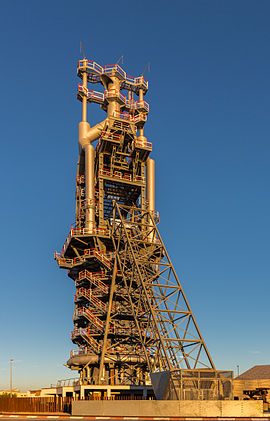
\includegraphics[width=4cm]{altoHorno.jpg}
    \caption{Alto horno.}
  \end{figure}

  Contamos con un modelo matemático, que explicaremos con más detalle en la próxima sección, que nos permite discretizar el dominio del problema y resolverlo por medio de un sistema de ecuaciones lineales. Por lo tanto, serán de interés para nosotros los métodos que permitan encontrar soluciones de este tipo de sistemas de manera computacional.

  Utilizaremos dos métodos diferentes para encarar el problema planteado: el método de Eliminación Gaussiana y el de Factorización LU. Ambos se valen del hecho de que un sistema de ecuaciones puede expresarse en forma matricial, y de que realizando ciertas operaciones sobre las filas de la matriz del sistema, puede obtenerse un sistema equivalente, que tiene las mismas soluciones. Más aún, puede probarse que todo sistema es equivalente a otro cuya matriz es triangular, y encontrar la solución de este tipo de sistemas es sumamente sencillo, utilizando los algoritmos de sustitución hacia adelante o sustitución hacia atrás.

  El método de \emph{Eliminación Gaussiana} itera sobre las columnas de la matriz, colocando ceros en todas las posiciones que se encuentran por debajo de la diagonal. Para hacer esto, en la $i$-ésima iteración, se resta a todas las filas a partir de la $i + 1$ un múltiplo de la fila $i$-ésima, con un factor elegido convenientemente. Esto asegura que, al completar el algoritmo, la matriz obtenida será triangular superior.

  En su forma más básica, el método falla si en alguna iteración se anula el elemento de la diagonal correspondiente a la columna sobre la que se está trabajando. Para salvar esta dificultad, se utiliza una técnica conocida como \emph{pivoteo}, que consiste en alterar el orden de las filas o de las columnas de la matriz. Sin embargo, como probaremos más adelante, la matriz asociada al sistema que estudiaremos tiene la particularidad de que el algoritmo de Eliminación Gaussiana puede aplicarse sin realizar pivoteo.

  El método de \emph{Factorización LU}, por su parte, aprovecha el hecho de que bajo ciertas condiciones, una matriz $A$ puede factorizarse como el producto de otras dos, en la forma $A = LU$, donde $L$ es triangular inferior con unos en la diagonal, y $U$ es triangular superior. De esta manera, el sistema $Ax=b$ puede reescribirse como $LUx=b$, y luego ser resuelto en dos etapas sencillas: si llamamos $y=Ux$, podemos resolver primero el sistema $Ly=b$ (aplicando sustitución hacia adelante, pues $L$ es triangular inferior), y una vez conocido el valor de $y$, resolver $Ux=y$ (aplicando esta vez sustitución hacia atrás), obteniendo así la solución del sistema original.

\clearpage
\section{Desarrollo}

    \subsection{Conceptos teóricos} \label{subsec:conceptos-teoricos}

        La resolución de \emph{sistemas de ecuaciones lineales} es un problema recurrente en el análisis numérico, ya que estos son útiles a la hora de modelar matemáticamente el comportamiento de problemas provenientes de diversas disciplinas, como la física y la ingeniería, para ser tratados en forma computacional. Es por eso que resulta de interés desarrollar algoritmos que permitan, de manera tan eficiente como sea posible, encontrar soluciones a estos sistemas.

        Un sistema de $m$ ecuaciones lineales con $n$ incógnitas tiene la forma
        \[ \left\lbrace \begin{matrix}
                a_{1,1} \, x_1 & + & a_{1,2} \, x_2 & + & \dots  & + & a_{1,n} \, x_n & = & b_1    \\
                a_{2,1} \, x_1 & + & a_{2,2} \, x_2 & + & \dots  & + & a_{2,n} \, x_n & = & b_2    \\
                \vdots         &   & \vdots         &   & \vdots &   & \vdots         &   & \vdots \\
                a_{m,1} \, x_1 & + & a_{m,2} \, x_2 & + & \dots  & + & a_{m,n} \, x_n & = & b_m    \\
        \end{matrix} \right. \]
        donde $a_{j,k}$ y $b_k$ (para $j = 1, \dots, m$; $k = 1, \dots, n$) son constantes reales. Por \emph{resolver} el sistema se entiende hallar un conjunto de valores para las incógnitas $x_1, \dots, x_n$ de forma que todas las ecuaciones se satisfagan simultáneamente.

        Una manera frecuente de representar un sistema de ecuaciones lineales, que será utilizada en este trabajo, es la matricial, que consiste en expresarlo en la forma
        \[ \mat{A}x = b \]
        donde 
        \[ \mat{A} = \left[ \begin{matrix} a_{1,1} & a_{1,2} & \dots  & a_{1,n} \\
                                           a_{2,1} & a_{2,2} & \dots  & a_{2,n} \\
                                           \vdots  & \vdots  & \ddots & \vdots  \\
                                           a_{m,1} & a_{m,2} & \dots  & a_{m,n} \\ \end{matrix} \right] \in \mathbb{R}^{m \times n} \qquad
        x = \left[ \begin{matrix} x_1 \\ x_2 \\ \vdots \\ x_n \end{matrix} \right] \in \mathbb{R}^n \qquad
        b = \left[ \begin{matrix} b_1 \\ b_2 \\ \vdots \\ b_m \end{matrix} \right] \in \mathbb{R}^m \]

        Dado un sistema de ecuaciones lineales, existe un conjunto de operaciones que, aplicadas sobre las ecuaciones, generan sistemas \emph{equivalentes}, es decir, que tienen las mismas soluciones. Más especificamente, estas operaciones son:
        \begin{enumerate}[label=(\alph*), nosep]
            \item Multiplicar una ecuación por una constante $\lambda \in \mathbb{R}$ no nula.
            \item Sumar a una ecuación el resultado de multiplicar otra por una constante $\lambda \in \mathbb{R}$.
            \item Intercambiar el orden de dos ecuaciones.
        \end{enumerate}

        Lo mismo vale para sistemas en forma matricial, si se consideran las operaciones análogas entre las filas de la matriz.

        Más aún, puede probarse que a partir de todo sistema puede obtenerse otro equivalente que se encuentra en forma \emph{triangular} o \emph{reducida} (ver \cite[p.~358]{burden}). Este resultado es importante porque, dado un sistema en forma triangular (superior o inferior), encontrar sus soluciones es sumamente sencillo, utilizando los algoritmos de \emph{sustitución hacia adelante} y el de \emph{sustitución hacia atrás}.

        Cabe destacar que un sistema de ecuaciones lineales puede no tener soluciones, tener solución única, o tener infinitas soluciones. En adelante se considerarán únicamente sistemas cuadrados (con igual número de ecuaciones que de incógnitas) cuya solución sea única, quedando los demás casos fuera del alcance de este trabajo. Bajo esta hipótesis, un sistema $\mat{A}x=b$ cumple la importante propiedad de que la matriz $\mat{A}$ es \emph{inversible}. En el caso de que $\mat{A}$ se encuentre en forma triangular, esto equivale a decir que no hay elementos nulos en su diagonal.

        El algoritmo de \emph{sustitución hacia adelante} considera un sistema de ecuaciones $\mat{L}x=b$, donde $\mat{L}$ es una matriz triangular inferior, y devuelve un vector $s$ solución del sistema. Lo hace aprovechando el hecho de, dado que la primer ecuación depende solamente de la primera incógnita, el valor de esta última puede ser despejado de forma inmediata; luego, sustituyendo este valor en la segunda ecuación, puede despejarse la segunda incógnita, y así sucesivamente hasta resolver el sistema completo. El algoritmo de \emph{sustitución hacia atrás} es análogo al anterior, pero considera un sistema de ecuaciones $\mat{U}x=b$, con $\mat{U}$ triangular superior, y realiza el proceso recorriendo las filas de la matriz en orden inverso, desde abajo hacia arriba. Ambos algoritmos tienen una complejidad cuadrática en la cantidad de incógnitas.

        \vspace{.5em}
        \begin{algorithm}[H]
            \caption{Sustitución hacia adelante} \label{alg:forward-substitution}
            \SetKwFunction{sustAdelante}{Sustitución hacia adelante}
            \KwData{$\mat{A} \in \mathbb{R}^{n \times n}, b \in \mathbb{R}^n$}
            \KwResult{$s \in \mathbb{R}^n$, solución del sistema $\mat{A}x=b$, considerando a $\mat{A}$ como una matriz triangular inferior, sin elementos nulos en la diagonal}
            \For{$j \gets 1$ \KwTo $n$}{
                $suma \gets 0$ \;
                \For{$k \gets 1$ \KwTo $j$}{
                    $suma \gets suma + s_k \cdot a_{j,k}$ \;
                }
                $s_j \gets \frac{b_j - suma}{a_{j,j}}$
            }
        \end{algorithm}
        \vspace{.5em}

        \vspace{.5em}
        \begin{algorithm}[H]
            \SetKwFunction{sustAtras}{Sustitución hacia atrás}
            \caption{Sustitución hacia atrás} \label{alg:backward-substitution}
            \KwData{$\mat{A} \in \mathbb{R}^{n \times n}, b \in \mathbb{R}^n$}
            \KwResult{$s \in \mathbb{R}^n$, solución del sistema $\mat{A}x=b$, considerando a $\mat{A}$ como una matriz triangular superior, sin elementos nulos en la diagonal}
            \For{$j \gets n$ \KwTo $1$}{
                $suma \gets 0$ \;
                \For{$k \gets j + 1$ \KwTo $n$}{
                    $suma \gets suma + s_k \cdot a_{j,k}$ \;
                }
                $s_j \gets \frac{b_j - suma}{a_{j,j}}$
            }
        \end{algorithm}
        \vspace{.5em}

        La sencillez con la que pueden resolverse sistemas cuando se encuentran en forma triangular es el principio en que se cimientan los dos métodos que se utilizarán en este trabajo, \emph{Eliminación Gaussiana} y \emph{Factorización LU}. La idea central de ambos es llevar el sistema de ecuaciones que pretende resolverse a otro equivalente en forma triangular, para así poder aplicar los algoritmos recién expuestos y encontrar su solución.

        \subsubsection{Eliminación Gaussiana}

            El método de \emph{Eliminación Gaussiana} itera sobre las columnas de la matriz, colocando ceros en todas las posiciones que se encuentran por debajo de la diagonal. Para hacer esto, en la $k$-ésima iteración, se resta a todas las filas a partir de la $k + 1$ un múltiplo de la fila $k$-ésima, con un factor elegido convenientemente.

            Más formalmente, supongamos que se pretende resolver el sistema $\mat{A}x = b$. Con la notación $\mat{A}^{(k)}$ se hará referencia a la matriz que se obtiene luego de aplicar $k$ iteraciones del algoritmo sobre $\mat{A}$, mientras que $\mat{A}_{k,*}$ denotará la $k$-ésima fila de la matriz $\mat{A}$.

            Inicialmente, se tiene que $\mat{A}^{(0)} = \mat{A}$. Luego, tras cada iteración, se obtiene:
            \[ \mat{A}^{(k)} = \left[ \begin{matrix}
                \mat{A}^{(k-1)}_{1,*} \\
                \vdots \\
                \mat{A}^{(k-1)}_{k,*} \\
                \mat{A}^{(k-1)}_{k+1,*} - m_{k+1,k} \mat{A}^{(k-1)}_{k,*} \\
                \vdots \\
                \mat{A}^{(k-1)}_{n,*} - m_{n,k} \mat{A}^{(k-1)}_{k,*} \\
            \end{matrix} \right] \]
            donde $m_{i,k} = \frac{a_{i,k}}{a_{k,k}}$. Esta elección de los multiplicadores tiene la particularidad de anular todos los elementos de la columna $k$ por debajo de la diagonal. Esto asegura que, al completar el algoritmo, luego de iterar sobre todas las columnas, la matriz obtenida será triangular superior.

            En su forma más básica, el método falla si, al comienzo de alguna iteración, es nulo el elemento de la diagonal correspondiente a la columna sobre la que se debe trabajar, es decir, si para algún $k = 1, \dots, n$ se cumple $a^{(k-1)}_{k,k} = 0$. Para salvar esta dificultad, se utiliza una técnica conocida como \emph{pivoteo}, que consiste en alterar el orden de las filas o de las columnas de la matriz. No obstante, bajo determinadas hipótesis, puede garantizarse que el algoritmo es aplicable sin necesidad de pivoteo; este será el caso en el contexto particular de este trabajo, por lo que no se entrará en más detalles acerca de esta técnica.

            \vspace{.5em}
            \begin{algorithm}[H]
                \caption{Eliminación Gaussiana} \label{alg:gaussian-elimination}
                \KwData{$\mat{A} \in \mathbb{R}^{n \times n}, b \in \mathbb{R}^n$}
                \KwResult{$s \in \mathbb{R}^n$, solución del sistema $\mat{A}x=b$}
                \For{$k \gets 1$ \KwTo $n$}{
                    \For{$j \gets k+1$ \KwTo $n$}{
                        $m \gets \frac{a_{j,k}}{a_{k,k}}$ \;
                        \For{$\ell \gets k$ \KwTo $n$}{
                            $a_{j,\ell} \gets a_{j,\ell} - m \cdot a_{k,\ell}$ \;
                        }
                        $b_j \gets b_j - m \cdot b_k$ \;
                    }
                }
                $s \gets$ \sustAtras{$\mat{A},b$} \;
            \end{algorithm}
        \vspace{.5em}

        \subsubsection{Factorización LU}

            El método de \emph{Factorización LU}, por su parte, aprovecha el hecho de que bajo ciertas condiciones, una matriz $\mat{A}$ puede factorizarse como el producto de otras dos, en la forma $\mat{A} = \mat{L}\mat{U}$, donde $\mat{L}$ es triangular inferior con unos en la diagonal, y $\mat{U}$ es triangular superior. De esta manera, el sistema $\mat{A}x=b$ puede reescribirse como $\mat{L}\mat{U}x=b$, y luego ser resuelto en dos etapas sencillas: si llamamos $y=\mat{U}x$, podemos resolver primero el sistema $\mat{L}y=b$ (aplicando sustitución hacia adelante, pues $\mat{L}$ es triangular inferior), y una vez conocido el valor de $y$, resolver $\mat{U}x=y$ (aplicando esta vez sustitución hacia atrás), obteniendo así la solución del sistema original.

            El pseudocódigo que se presenta como Algoritmo \ref{alg:lu-decomposition} muestra el procedimiento a seguir para encontrar la factorización LU de una matriz, asumiendo que dicha factorización existe. El mismo genera como salida una única matriz $\mat{B}$ que contiene tanto los coeficientes no nulos de $\mat{L}$ como los de $\mat{U}$; esta es una optimización destinada a la implementación, con el objetivo de mejorar su eficiencia evitando el almacenamiento de información redundante.

            {\color{red}
                IMPORTANTE: REVISAR EL PSEUDOCÓDIGO, PORQUE CREO QUE ESTÁ MAL
            }

            \vspace{.5em}
            \begin{algorithm}[H]
                \caption{Factorización LU} \label{alg:lu-decomposition}
                \KwData{$\mat{A} \in \mathbb{R}^{n \times n}$}
                \KwResult{$\mat{B} \in \mathbb{R}^{n \times n}$, tal que los elementos ubicados por encima de y en la diagonal forman una matriz triangular superior $\mat{U}$, y los ubicados por debajo de la misma, completados con unos en la diagonal, forman una matriz triangular inferior $\mat{L}$, con $\mat{L}\mat{U}=\mat{A}$}
                \For{$k \gets 1$ \KwTo $n$}{
                    \For{$j \gets k+1$ \KwTo $n$}{
                        $m \gets \frac{a_{j,k}}{a_{k,k}}$ \;
                        $b_{j,k} \gets m$ \;
                        \For{$\ell \gets k+1$ \KwTo $n$}{
                            $b_{j,\ell} \gets a_{j,\ell} - m \cdot a_{k,\ell}$ \;
                        }
                    }
                }
            \end{algorithm}
            \vspace{.5em}

            En cuanto a las hipótesis que permiten asegurar la existencia de la factorización LU de una matriz, resultará de utilidad el siguiente resultado, cuya demostración puede encontrarse en \cite[p.~403]{burden}.

            \begin{prop} \label{prop:EG sin pivoteo implica LU}
                Si una matriz $\mat{A} \in \mathbb{R}^{n \times n}$ es tal que el sistema $\mat{A}x=b$ ($b \in \mathbb{R}^{n}$) puede ser resuelto aplicando Eliminación Gaussiana sin pivoteo, entonces $\mat{A}$ puede ser factorizada de la forma $\mat{A}=\mat{L}\mat{U}$, donde $\mat{U}$ es una matriz triangular superior y $\mat{L}$ es una matriz triangular inferior con unos en la diagonal.
            \end{prop}

    \subsection{Modelado del sistema}

        Para resolver el problema presentado en la Introducción, se considerará una sección horizontal del horno, como puede verse en la Figura \ref{fig:seccion-horno}. Se denominará $r_e \in \mathbb{R}_{>0}$ al radio exterior y $r_i \in \mathbb{R}_{>0}$ al radio interior de la pared del horno. Para cada punto, se considerarán sus coordenadas polares $(r, \theta)$ con origen en el centro del horno, llamando $T(r, \theta)$ a la temperatura en dicho punto. Se considerará conocido el valor (constante) de la temperatura en el interior del horno, \[ T_i = T(r, \theta) \qquad (\forall \, r \in [0, r_i], \, \theta \in [0, 2 \pi)) \] como así también el correspondiente a los puntos de la pared externa, \[ T_e(\theta) = T(r_e, \theta) \]
        
        \begin{figure}[h]
          \centering

          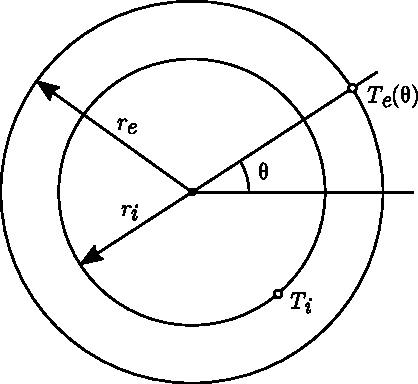
\includegraphics{imagenes/seccion-horno.pdf}

          \caption{Sección horizontal del horno.}
          \label{fig:seccion-horno}
        \end{figure}

        En el estado estacionario, la temperatura $T$ satisface la ecuación del calor:
        \begin{equation} \label{eq:calor}
            \frac{\partial^2 T(r, \theta)}{\partial r^2} + \frac{1}{r} \frac{\partial T(r, \theta)}{\partial r} + \frac{1}{r^2} \frac{\partial^2 T(r, \theta)}{\partial \theta^2} = 0
        \end{equation}

        No obstante, esta ecuación plantea un modelo continuo para estudiar el problema. Para poder tratar computacionalmente el mismo, se hace necesario discretizar su dominio, considerando una cantidad finita de puntos del mismo. Con este fin, se adoptará una partición del sector interno de la pared del horno, tal y como ilustra la Figura \ref{fig:discretizacion}, en $m + 1$ radios equidistantes 
        \[ r_i = r_0 < r_1 < \dots < r_m = r_e \text{, \qquad con } r_j - r_{j-1} = \Delta r \text{ para } j = 1, \dots, m+1 \]
        y en $n$ ángulos iguales
        \[ 0 = \theta_0 < \theta_1 < ... < \theta_n = 2\pi \text{, \qquad con } \theta_k - \theta_{k-1} = \Delta \theta \text{ para } k = 1, \dots, n \]

        \begin{figure}[h]
          \centering

          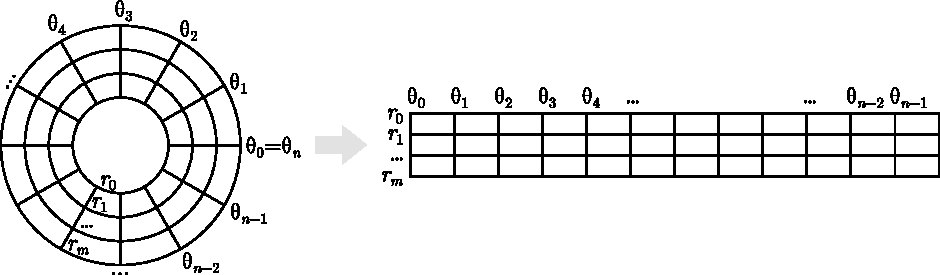
\includegraphics{imagenes/discretizacion.pdf}

          \caption{Discretización del dominio del problema.}
          \label{fig:discretizacion}
        \end{figure}

        Nuestro objetivo es calcular el valor de la temperatura en todos los puntos de la discretización $t_{j,k} = T(r_j, \theta_k)$ para $j = 0, \dots, m$ y $k = 0, \dots, n-1$. Gracias a los datos disponibles sobre las condiciones de borde, conocemos el valor de la temperatura en los puntos de las paredes externa e interna: $t_{m,k} = T_e(\theta_k)$ y $t_{0,k} = T_i$, para todo $k = 0, \dots, n-1$.

        Para discretizar el problema continuo planteado por la ecuación (\ref{eq:calor}), y así obtener el valor en los puntos internos de la pared, pueden utilizarse las siguientes fórmulas de diferencias finitas
        \begin{align*}
            \frac{\partial^2 T(r, \theta)}{\partial r^2}(r_j, \theta_k) &\cong \frac{t_{j-1,k} - 2 t_{jk} + t_{j+1,k}}{(\Delta r)^2} \\
            \frac{\partial T(r, \theta)}{\partial r}(r_j, \theta_k) &\cong \frac{t_{j,k} - t_{j-1,k}}{\Delta r} \\
            \frac{\partial^2 T(r, \theta)}{\partial \theta^2}(r_j, \theta_k) &\cong \frac{t_{j,k-1} - 2 t_{jk} + t_{j,k+1}}{(\Delta \theta)^2} 
        \end{align*}
        que, reemplazadas en la ecuación (\ref{eq:calor}), permiten obtener una formulación de la temperatura en estos puntos en función de sus cuatro puntos vecinos más próximos. Más específicamente, para $1 \leq j < m,\ 0 \leq k < n$, se tiene que:
        \begin{multline} \label{eq:calor-discreto}
            \Phi(j,k) = \left( \frac{1}{(\Delta r)^2} - \frac{1}{r \Delta r} \right) t_{j-1,k} +
                \left( \frac{1}{r^2(\Delta \theta)^2} \right) t_{j,k-1} + \\
                \left( - \frac{2}{(\Delta r)^2} + \frac{1}{r \Delta r} - \frac{2}{r^2(\Delta \theta)^2} \right) t_{j,k} +
                \left( \frac{1}{r^2(\Delta \theta)^2} \right) t_{j,k+1} +
                \left( \frac{1}{(\Delta r)^2} \right) t_{j+1,k} = 0
        \end{multline}

        De esta manera, podemos reunir la información de la que disponemos sobre el problema discreto en un sistema de $(m+1)n$ ecuaciones con $(m+1)n$ incógnitas, cada una de ellas el valor de la temperatura en un punto de la discretización, es decir, $t_{j,k}$ para algún $j = 0, \dots, m$, $k = 0, \dots, n-1$. En otras palabras, el problema de calcular la temperatura en todos los puntos de la discretización se traduce en la resolución del siguiente sistema de ecuaciones lineales:

        \begin{equation} \label{eq:sistema}
            \begin{cases}
                t_{0,k} = T_i
                    & \text{para } 0 \leq k < n \\
                0 = \Phi(j,k)
                    & \text{para } 1 \leq j < m,\ 0 \leq k < n \\
                t_{m,k} = T_e(\theta_k)
                    & \text{para } 0 \leq k < n
            \end{cases}
        \end{equation}

        Como puede verse, cada ecuación del sistema está asociada directamente al cálculo de la temperatura en uno de los puntos de la discretización, es decir, a una de las incógnitas.

        A partir de ahora, se considerará la representación matricial del sistema, $\mat{A}x=b$, con $\mat{A} \in \mathbb{R}^{(m+1)n \times (m+1)n}$ y $b \in \mathbb{R}^{(m+1)n}$. Para construir la matriz $\mat{A}$, se ordenan tanto las incógnitas $t_{j,k}$ como las ecuaciones asociadas a ellas, primero de acuerdo al radio ($j$) y luego de acuerdo al ángulo ($k$). Esto significa que los coeficientes correspondientes a la incógnita $t_{j,k}$ se encontrarán en la columna $(m+1)j + k + 1$, y a la ecuación asociada al cálculo de esta incógnita le corresponderá la fila con el mismo índice.

        Puede notarse que las primeras $n$ filas y las últimas $n$ filas de la matriz, correspondientes a los puntos de la pared interna y externa del horno, respectivamente, contendrán un $1$ en la diagonal y $0$ en todas las demás posiciones, dado que allí la temperatura ya es conocida y no depende de ningún otro punto. En las demás filas, correspondientes a los puntos internos de la pared del horno, la temperatura depende solamente del valor de la misma en los cuatro vecinos más próximos; esto provoca que los coeficientes no nulos se encuentren confinados a un entorno relativamente reducido de la diagonal de la matriz. Más precisamente, todos los coeficientes que se encuentran fuera de una banda de ancho $n$ hacia ambos lados de la diagonal son nulos, i.e. $a_{p,q} = 0$ siempre que $\vert p - q \vert > n$. En otras palabras, la matriz construida es \emph{banda} $n, n$; este hecho puede observarse claramente en la Figura \ref{fig:matriz-banda}.

        \begin{figure}[h]
          \centering

          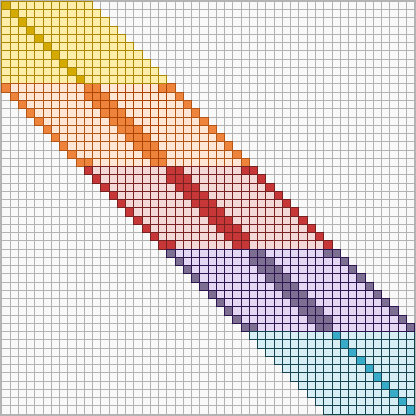
\includegraphics{imagenes/matriz-banda.pdf}

          \caption{Matriz asociada al sistema con $m = 4$ y $n = 10$. Aparecen resaltados los coeficientes no nulos.}
          \label{fig:matriz-banda}
        \end{figure}

    \subsection{Aplicabilidad de los métodos elegidos}

        Los métodos numéricos ya presentados no son aplicables a la hora de resolver cualquier sistema de ecuaciones lineales, sino que requieren que este satisfaga determinadas hipótesis. Por este motivo, es necesario demostrar que estas se cumplen en el caso particular del sistema que modela el problema a resolver en este trabajo.

        El objetivo es demostrar que tanto el método de Eliminación Gaussiana (sin pivoteo) como el de Factorización LU pueden aplicarse para resolver el sistema planteado en la sección anterior. Sin embargo, de lo enunciado en la Proposición \ref{prop:EG sin pivoteo implica LU} (sección \ref{subsec:conceptos-teoricos}) se desprende que basta con probar la aplicabilidad del primero de ellos. A continuación se procederá a introducir una definición y demostrar un lema, que luego se utilizarán durante la demostración.

        \begin{defi}
            Sea $\mat{A} \in \mathbb{R}^{n \times n}$. $\mat{A}$ se dice \emph{diagonal dominante} (por filas, de manera no estricta) si cada uno de los elementos de su diagonal es mayor o igual, en módulo, que la suma de los módulos de todos los demás coeficientes presentes en la misma fila. Es decir, si
            \[ \vert a_{j,j} \vert \geq \sum_{\substack{k=1 \\ k \neq j}}^n \vert a_{j,k} \vert \qquad \text{para todo $j = 1, \dots, n$} \]
        \end{defi}

        \begin{lema}
            \label{lema:EG conserva diagonal dominante}
            Sea $\mat{A}^{(0)} = \mat{A} \in \mathbb{R}^{n \times n}$ una matriz diagonal dominante, con $\mat{A}_{1,1} \neq 0$, y $\mat{A}^{(1)}$ el resultado de aplicar un paso de Eliminación Gaussiana (sin pivoteo) sobre $\mat{A}$. Entonces $\mat{A}^{(1)}$ es diagonal dominante.
        \end{lema}
        \begin{proof}
            Se considerará la fila $j$-ésima de $\mat{A}^{(1)}$, para ver que $\left \vert a^{(1)}_{j,j} \right \vert \geq \sum_{\substack{k = 1 \\ k \neq j}}^n \left \vert a^{(1)}_{j,k} \right \vert$. Se tiene que
            \[ \left \vert a^{(1)}_{j,j} \right \vert = \left \vert a_{j,j} - \frac{a_{j,1}}{a_{1,1}} a_{1,j} \right \vert
                \qquad \text{y} \qquad
            \sum_{\substack{k = 1 \\ k \neq j}}^n \left \vert a^{(1)}_{j,k} \right \vert
                = \sum_{\substack{k = 2 \\ k \neq j}}^n \left \vert a_{j,k} - \frac{a_{j,1}}{a_{1,1}} a_{1,k} \right \vert \]

            Luego,

            \[ \begin{split}
                \sum_{\substack{k = 1 \\ k \neq j}}^n \left \vert a^{(1)}_{j,k} \right \vert
                &= \sum_{\substack{k = 2 \\ k \neq j}}^n \left \vert a_{j,k} - \frac{a_{j,1}}{a_{1,1}} a_{1,k} \right \vert \\
                &\leq \sum_{\substack{k = 2 \\ k \neq j}}^n \vert a_{j,k} \vert + \left \vert \frac{a_{j,1}}{a_{1,1}} \right \vert \sum_{\substack{k = 2 \\ k \neq j}}^n \vert a_{1,j} \vert \\
                &\leq \left( \vert a_{j,j} \vert - \vert a_{j,1} \vert \right) + \left \vert \frac{a_{j,1}}{a_{1,1}} \right \vert \left( \vert a_{1,1} \vert - \vert a_{1,j} \vert \right) \\
                &= \vert a_{j,j} \vert - \left \vert \frac{a_{j,1}}{a_{1,1}} \right \vert \vert a_{1,j} \vert \\
                &\leq \left \vert a_{j,j} -  \frac{a_{j,1}}{a_{1,1}} a_{1,j} \right \vert = \left \vert a^{(1)}_{j,j} \right \vert \qedhere
            \end{split} \]
        \end{proof}

        Contando con estos resultados, se probará que el sistema construido en la sección anterior, tal y como fue expuesto en (\ref{eq:sistema}), puede ser resuelto aplicando Eliminación Gaussiana sin pivoteo. La demostración tendrá dos etapas:
        \begin{enumerate}
            \item Demostrar que la matriz $\mat{A} \in \mathbb{R}^{(m+1)n \times (m+1)n}$ asociada al sistema es diagonal dominante.
            \item Demostrar, a partir de este hecho y en forma inductiva, que todas las iteraciones del algoritmo de Eliminación Gaussiana están bien definidas, sin utilizar pivoteo.
        \end{enumerate}

        Para ver que la matriz $\mat{A}$ es diagonal dominante, se verificará separadamente que la definición se cumple para las filas correspondientes a los bordes de la pared del horno (primeras $n$ filas y últimas $n$ filas) y para las correspondientes a los puntos internos.

        \begin{enumerate}[label=(\roman*)]
            \item Para $p = 1, \dots, n$ y para $p = mn + 1, \dots, (m+1)n$, la fila $p$-ésima corresponde a un punto del borde de la pared del horno. Como ya se señaló anteriormente, en estas filas hay un $1$ en los lugares correspondientes a la diagonal, mientras que los demás coeficientes son nulos. Por lo tanto, se sigue trivialmente que, para $p = 1, \dots, n, mn + 1, (m+1)n$:
            \[ \vert a_{p,p} \vert = 1 \geq 0 = \sum_{\substack{q=1 \\ q \neq p}}^{(m+1)n} \vert a_{p,q} \vert \]

            \item Para $p = n + 1, \dots, mn$, la fila $p$-ésima corresponde a un punto interno de la pared. Es decir, representa a una ecuación del tipo $\Phi(j,k) = 0$, con $j = 1, \dots, m - 1$ y $k = 0, \dots, n - 1$. Luego, esta fila contiene solo 5 coeficientes no nulos.

            El coeficiente que aparece en la diagonal es el correspondiente a la variable $t_{j,k}$. Entonces:
            \[ \begin{split}
                \vert a_{p,p} \vert &= \left \vert - \frac{2}{(\Delta r)^2} + \frac{1}{r \Delta r} - \frac{2}{r^2 (\Delta \theta)^2} \right \vert \\
                &= \left \vert - \frac{1}{(\Delta r)^2} + \frac{1}{r \Delta r} - \frac{2}{r^2 (\Delta \theta)^2} - \frac{1}{(\Delta r)^2} \right \vert \\
                &= \left \vert - \frac{r - \Delta r}{r (\Delta r)^2} - \frac{2}{r^2 (\Delta \theta)^2} - \frac{1}{(\Delta r)^2} \right \vert \\
                &= \left \vert \frac{r - \Delta r}{r (\Delta r)^2} + \frac{2}{r^2 (\Delta \theta)^2} + \frac{1}{(\Delta r)^2} \right \vert
            \end{split} \]

            Dado que $r_i, \Delta r > 0$ y $j \geq 1$, se cumple que
            \[ r - \Delta r = (r_i + j \Delta r) - \Delta r = r_i + (j - 1) \Delta r > 0\]
            de donde se desprende que todos los términos que aparecen dentro del módulo son positivos, y por lo tanto
            \[ \vert a_{p,p} \vert = \frac{r - \Delta r}{r (\Delta r)^2} + \frac{2}{r^2 (\Delta \theta)^2} + \frac{1}{(\Delta r)^2} \]

            Por otro lado, si se suman los módulos de los demás coeficientes de la fila, se obtiene:
                \[ \begin{split}
                    \sum_{\substack{q=1 \\ q \neq p}}^{(m+1)n} \vert a_{p,q} \vert &= \left \vert \frac{1}{(\Delta r)^2} - \frac{1}{r \Delta r} \right \vert + 2 \left \vert \frac{1}{r^2 (\Delta \theta)^2} \right \vert + \left \vert \frac{1}{(\Delta r)^2} \right \vert \\
                    &= \left \vert \frac{r - \Delta r}{r (\Delta r)^2} \right \vert + \frac{2}{r^2 (\Delta \theta)^2} + \frac{1}{(\Delta r)^2} \\
                    &= \frac{r - \Delta r}{r (\Delta r)^2} + \frac{2}{r^2 (\Delta \theta)^2} + \frac{1}{(\Delta r)^2} = \vert a_{p,p} \vert
                \end{split} \]
        \end{enumerate}

        De todo lo anterior, se sigue que $\mat{A}$ es diagonal dominante de forma no estricta, como se quería demostrar.

        \begin{obs} \label{obs:Diagonal de A sin ceros}
        De la demostración anterior se desprende que para todo $p = 1, \dots, (m+1)n$, $\vert a_{p,p} \vert > 0$; es decir, la diagonal de $\mat{A}$ no contiene ceros.
        \end{obs}

        Por último, se debe probar que las $(m+1)n$ iteraciones del algoritmo de Eliminación Gaussiana necesarias para resolver el sistema pueden aplicarse, y que no es necesario utilizar pivoteo. La idea será demostrar que, para todo $u \leq (m+1)n$, pueden aplicarse $u$ iteraciones de Eliminación Gaussiana sobre $\mat{A}$ sin pivoteo, y que además, la matriz $\mat{A}^{(u)}$ que resulta de este proceso es diagonal dominante, y su fila $u + 1$ es no nula. La demostración será por inducción en $u$.

        \begin{enumerate}[label=(\roman*)]
            \item \strong{Caso base.} Como $a_{1,1} = 1$ no es nulo, se puede aplicar la primera iteración de Eliminación Gaussiana sin realizar pivoteo. Dado que $\mat{A}$ es diagonal dominante, por el Lema \ref{lema:EG conserva diagonal dominante}, la matriz $]mat{A}^{(1)}$ obtenida también será diagonal dominante. Además, se sabe que $a_{1,2} = 0$, por lo que la primera iteración del algoritmo no afectará al coeficiente $a_{2,2}$, que era necesariamente no nulo (ver Observación \ref{obs:Diagonal de A sin ceros}). Luego, la segunda fila de $\mat{A}^{(1)}$ será no nula.
                    
            \item \strong{Paso inductivo.} Por hipótesis inductiva, la matriz $\mat{A}^{(u-1)}$, obtenida tras aplicar $u-1$ pasos de Eliminación Gaussiana sobre $\mat{A}$, es diagonal dominante y su $u$-ésima fila es no nula. Esto implica que $a^{(u-1)}_{u,u} \neq 0$.

            Nótese que es posible escribir a $\mat{A}^{(u-1)}$ por bloques de la siguiente manera:
            \[ \mat{A}^{(u-1)} = \left( \begin{matrix} \mat{U}_{u-1} & \mat{B} \\ \mat{0} & \widetilde{\mat{A}}_{u-1} \end{matrix} \right) \]
            donde las matrices $\mat{U}_{u-1} \in \mathbb{R}^{(u-1)\times(u-1)}$ y $\widetilde{\mat{A}}_{u-1} \in \mathbb{R}^{((m+1)n-u+1)\times((m+1)n-u+1)}$ son trivialmente diagonal dominantes.

            Se puede ver que realizar el paso $u$-ésimo del algoritmo de Eliminación Gaussiana sobre $\mat{A}$ equivale a realizar el primer paso de este algoritmo sobre $\widetilde{\mat{A}}_{u-1}$, manteniendo intacto el resto de la matriz. Dado que $a^{(u-1)}_{u,u} \neq 0$, esto puede realizarse sin pivoteo, y del Lema \ref{lema:EG conserva diagonal dominante} se sigue que el resultado de este proceso será diagonal dominante, lo cual implica directamente que también lo será $\mat{A}^{(u)}$.

            Solo resta probar que la fila $u+1$ de la matriz $\mat{A}^{(u)}$ es no nula.
            \begin{enumerate}[label=(\alph*)]
                \item Si la fila $u + 1$ corresponde a uno de los puntos externos de la pared del horno, es decir, si $1 \leq u+1 \leq n$ o $mn < u + 1 \leq (m+1)n$, entonces tendrá un $1$ en la diagonal y $0$ en las demás posiciones, por lo que no se verá afectada por el algoritmo de Eliminación Gaussiana.
                \item En caso contrario, la fila corresponde a una de los puntos internos de la pared, representando a una de las ecuaciones del tipo $\Phi(j,k) = 0$, para ciertos $j = 1, \dots, m - 1$ y $k = 0, \dots, n - 1$. Puntualmente, por la forma en la que se construye la matriz del sistema, el elemento $a_{u+1,u+1+n}$ es el coeficiente de la variable $t_{j,k+1}$ en dicha ecuación, que es necesariamente no nulo. Por otra parte, como la matriz $\mat{A}$ es \emph{banda} $n, n$, todos los elementos de la columna $u+1$ que se encuentran por encima de $a_{u+1,u+1+n}$ deben ser nulos. Esto quiere decir que ninguna de las iteraciones ya ejecutadas de Eliminación Gaussiana modificaron este coeficiente, y por lo tanto, sigue siendo no nulo.
            \end{enumerate}
        \end{enumerate}

    \subsection{Interpretación de los resultados}

        \subsubsection{Estimación de la posición de la isoterma crítica}

            Además de contar con métodos para la resolución del sistema, la resolución del problema requirió la elaboración con criterios para interpretar los resultados obtenidos. Uno de los aspectos necesarios fue la posibilidad de estimar el conjunto de puntos en el interior del horno que se encontraban a una temperatura dada, es decir, la posición de la isoterma correspondiente.

            Como criterio general, se decidió evaluar independientemente los valores encontrados para cada uno de los ángulos de la discretización, procurando estimar, para cada uno de estos radios, el radio del punto cuya temperatura fuera la buscada. Más formalmente, dada una temperatura $c$, se buscó calcular un vector $i = (i_0, \dots, i_{n-1})$, donde cada $i_k$ es tal que $T(i_k, \Theta_k) = c$.

            Un análisis sencillo de las funciones involucradas permitió arribar a la conclusión de que, a lo largo de cada ángulo, la temperatura se comportaría de forma monótona, por lo que en general el valor $i_k$ estaría bien definido; más aún teniendo en cuenta que, dado el contexto de aplicación, cabe esperar temperaturas muy superiores en el interior que en el exterior del horno. En el caso excepcional de que la temperatura se mantuviera constante a lo largo del ángulo, debería procurarse elegir el más externo de los puntos válidos, para no afectar así la estimaciones posteriores acerca del riesgo de la estructura, que dependen de la cercanía de la isoterma a la pared.

            Se evaluaron tres técnicas diferentes para la estimación de los valores $i_k$, que se enumeran a continuación:

            \begin{enumerate}
                \item Para cada ángulo $\theta_k$, elegir entre los radios de la discretización aquel cuya temperatura fuera más próxima a la temperatura crítica $c$. Este criterio es sumamente sencillo, pero se ve seriamente limitado al tomar en cuenta únicamente puntos de la discretización; esto podría causar que se viera seriamente afectado si la misma tuviera una baja granularidad en cuanto a cantidad de radios considerados. Peor aún, la isoterma real podría estar más cerca de la pared externa del horno que la estimada con este método, evitando, especialmente en conjunción con el problema recién mencionado, que se detecten situaciones de riesgo.
                \item Para cada ángulo $\theta_k$, determinar el más externo de los radios de la discretización cuya temperatura fuera mayor o igual que la temperatura crítica $c$, y elegir luego como $i_k$ el radio de la discretización inmediatamente exterior. Esto equivale a seleccionar el más interno de los radios de la discretización tal que su temperatura y las de todos los radios más externos fuera menor a $c$, es decir 
                \[ i_k = \min \left\lbrace r_j \; \vert \; 0 \leq j \leq m \; \land \; t_{j',k} < c \, (\forall \, j' = j, \dots, m) \right\rbrace \]
                La ventaja de este método es que asegura que la isoterma nunca se encontrará más cerca de la pared externa que el resultado arrojado, garantizando que se detectarán todas las posibles situaciones de riesgo.
                \item Para cada ángulo $\theta_k$, considerar $\tilde{r_j}$, el más externo de los radios de la discretización con temperatura mayor o igual a $c$. Luego, sabiendo que la isoterma buscada se encontrará entre este radio y el inmediatamente exterior, aproximar la variación de la temperatura en los puntos intermedios mediante una función lineal y utilizar esta aproximación para estimar la posición de la isoterma. Más precisamente
                \[ i_k = r_j + \Delta r \left(\frac{c - t_{j,k}}{t_{j+1,k} - t_{j,k}} \right) \]
            \end{enumerate}

            Finalmente, decidimos aplicar este último criterio, porque consideramos que brinda información más precisa que los otros dos, al tener en cuenta el valor la diferencia de temperatura entre los puntos de la discretización más cercanos a la isoterma buscada y la isoterma en si misma, información que los dos primeros métodos descartan. De esta manera, nos permite detectar situaciones de riesgo que con el primer método pasarían desapercibidas, pero evitando la generación de falsos positivos que provocaría el segundo método, que es mucho más estricto.

        \subsubsection{Cálculo del índice de peligrosidad}

            Para elegir la medida de peligrosidad lo que hacemos es tomar de todos los valores por los que pasa la isoterma el mas próximo a la pared externa del alto horno. A ese valor lo dividimos por el radio externo, dando así la relación entre la distancia mas cercana a la pared externa de la isoterma y la distancia total.
            Este es un numero entre 1 y 0 donde 0 es el centro del horno y 1 es la pared externa. Cuanto mas cercano a 1 sea el valor, mas peligro de colapsar tiene.

    \subsection{Implementación}

        Los dos métodos utilizados fueron implementados en lenguaje C++. Para la representación interna de las matrices se utiliza el tipo \texttt{vector}, proporcionado por la biblioteca estándar de C++. Se utilizó el mecanismo de clases del lenguaje para mejorar la organización del código, proporcionando métodos que implementan los diversos algoritmos ya presentados: sustitución hacia adelante y hacia atrás, Eliminación Gaussiana y Factorización LU.

        Adicionalmente, se incorporaron a la implementación funciones para estimar, en función de la salida del algoritmo, la posición de la isoterma según las tres técnicas ideadas, como así también para calcular el índice de peligrosidad.

        Un aspecto que se presentó durante la etapa de implementación fue la posibilidad de optimizar su rendimiento aprovechando la información disponible sobre el sistema a resolver. Puntualmente, el hecho de que la matriz con la que se trabaja es \emph{banda} permite mejorar tanto la complejidad temporal como espacial del programa, evitando almacenar y procesar una gran cantidad de coeficientes de la matriz cuando ya se sabe que estos son nulos. No obstante, se decidió omitir esta posible optimización, ya que se contaba con un tiempo limitado y se consideró preferible priorizar la realización de pruebas experimentales.

\clearpage
 \subsection{Experimentación y discusión}

    A continuación, se presentan las pruebas experimentales que se realizaron con el fin de evaluar y comparar los diferentes métodos ya presentados, junto con los resultados obtenidos y una discusión de los mismos.

    Todos los experimentos se ejecutaron en las computadoras del laboratorio 4 del Departamento de Computación (FCEN - UBA). 

    \subsubsection*{Experimento 1: Tiempo según granularidad} 

      \subsubsection*{Presentación}
        El objetivo de este experimento es observar como varían los tiempos de ejecución al resolver sistemas con mismas temperaturas pero diferente granularidad, y modificando el método utilizado. 
        Hacemos el mismo experimento dos veces, uno para cada uno de los métodos numéricos. Manteniendo las temperaturas constantes, variamos cantidad de particiones de los ángulos dejando la de los radios intacta. Calculamos la solución del sistema para cada una de las distintas granularidades y comparamos los tiempos que toman las diferentes ejecuciones. Repetimos esto mismo, ahora variando las particiones de los radios. Luego tomamos el otro método numérico y volvemos a iniciar el experimento. 

      \subsubsection*{Datos}
        Para ambos casos, se construyeron escenarios de prueba con los siguientes parámetros: $r_i = 30$, $r_e = 60$, $T_i = 1500$, $iso = 500$. La temperatura externa se consideró constante, con $T_e(\theta) = 50$ para todo $\theta$. En ambos casos las pruebas se realizaron utilizando primero el método de Eliminación Gaussiana y luego el de Factorización LU, y los tiempos de ejecución se tomaron en segundos, utilizando la librería \texttt{ctime} de \texttt{C++}. Para las pruebas se omitió realizar la estimación de la posición de la isoterma, limitándose a resolver el sistema por el método elegido ya que el cálculo de la isoterma es idéntico en ambos algoritmos y no afectará al análisis del tiempo de ejecución. 
      
          \paragraph{Caso A} 
          Se realizaron pruebas variando la cantidad de ángulos de la discretización, con $m + 1 = 30$ y $n = 10, 30, 50, 70, 90$. Se puede encontrar en los archivos adjuntos llamados exp1a-$n$.in la instancia pasada por parámetro.

          \paragraph{Caso B} 
          Se realizaron pruebas variando la cantidad de radios de la discretización, con $n = 60$ y $m+1 = 10, 30, 50, 70$. Se puede encontrar en los archivos adjuntos llamados exp1b-$m+1$.in la instancia pasada por parámetro.

      \subsubsection*{Hipótesis}
        La complejidad del algoritmo es cúbico en el tamaño de la entrada. Como solo variamos la granularidad del radio o del ángulo (dejando el otro constante) entonces en ambos casos suponemos que el tiempo de ejecución va a ser cubico con relación a la granularidad de la entrada. 


      \subsubsection*{Resultados}

      \subsubsection*{Caso A}
       
        {\centering \begin{tabular}{cc}
           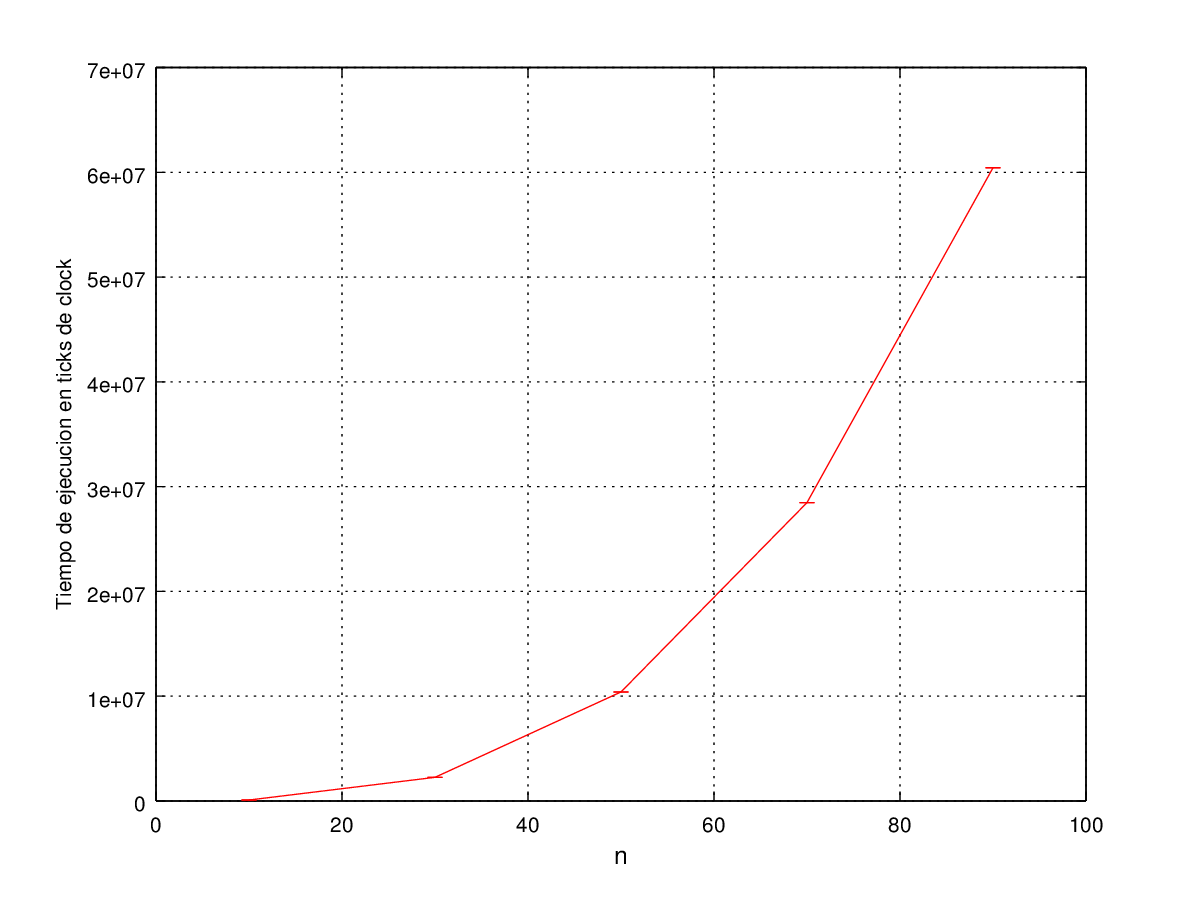
\includegraphics[height=5cm]{graficos/exp1/exp1-angulos0.png} & 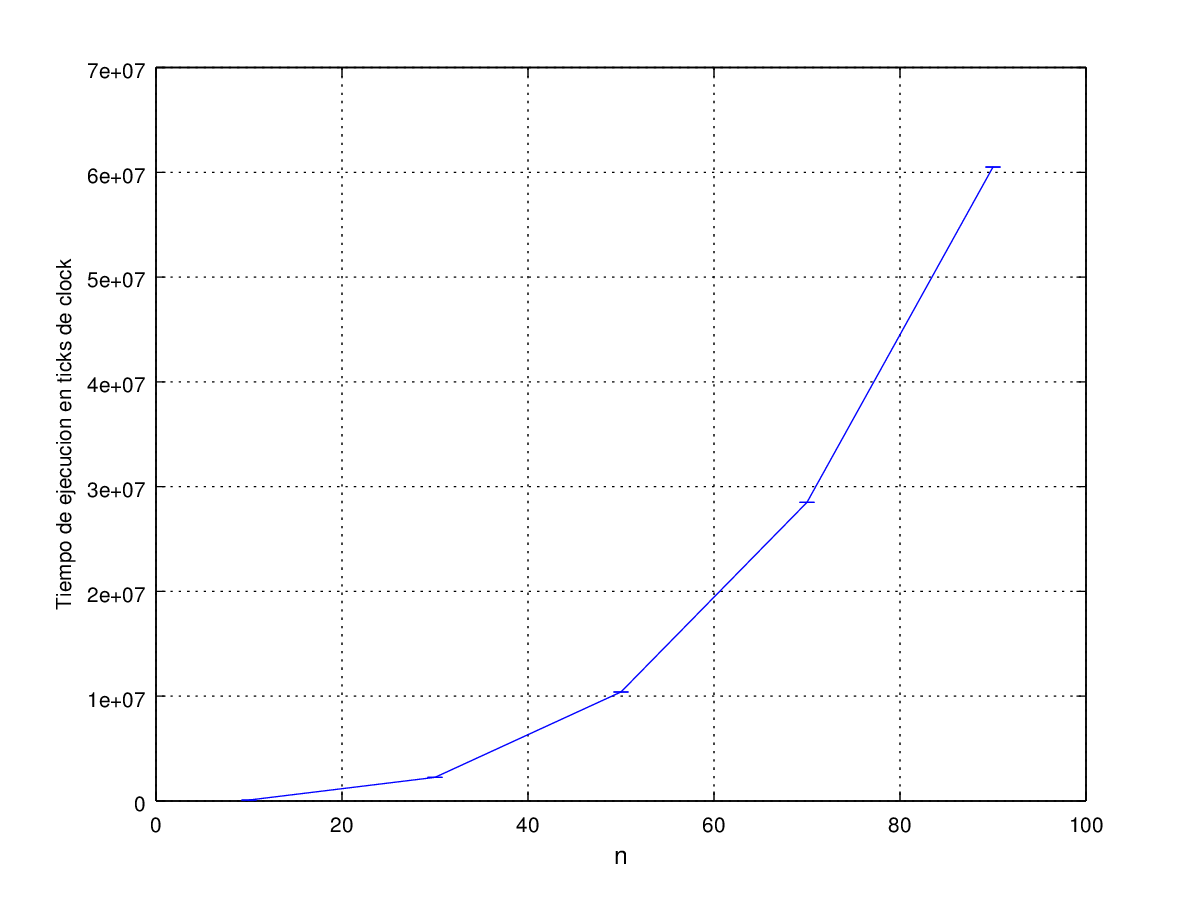
\includegraphics[height=5cm]{graficos/exp1/exp1-angulos1.png} \\
          {\small Eliminación Gaussiana} &
          {\small Factorización LU} \\
         \end{tabular}}


    \subsubsection*{Caso B}
        
        {\centering \begin{tabular}{cc}
           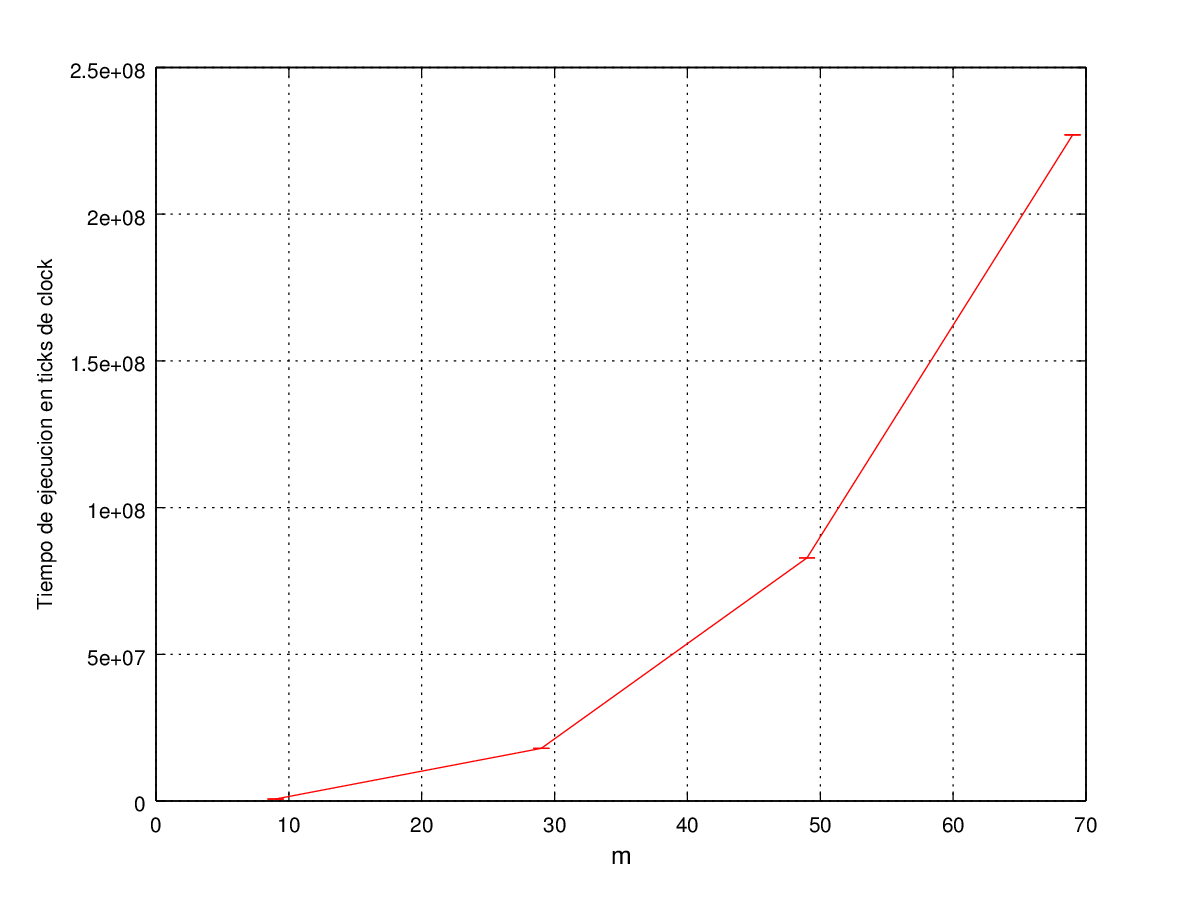
\includegraphics[height=5cm]{graficos/exp1/exp1-radios0.png} & 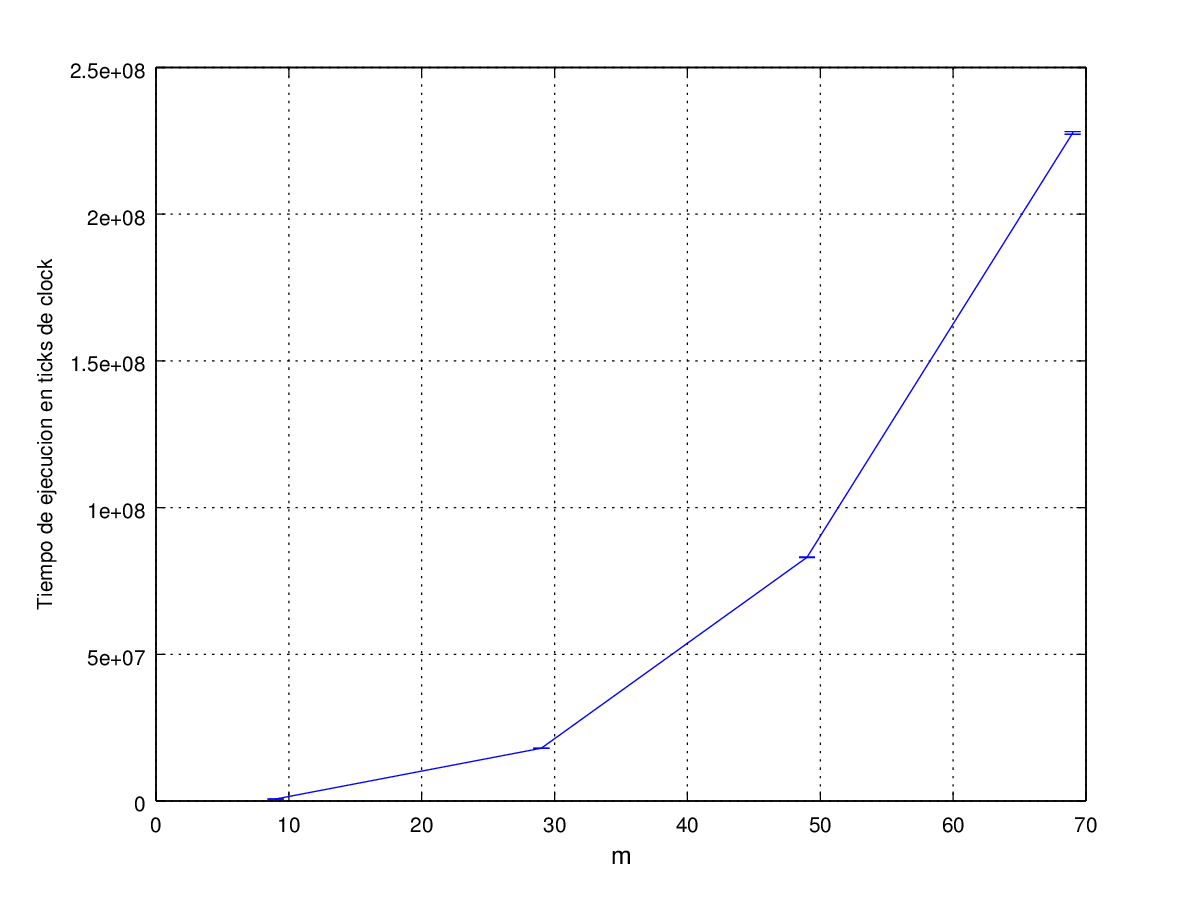
\includegraphics[height=5cm]{graficos/exp1/exp1-radios1.png} \\
          {\small Eliminación Gaussiana} &
          {\small Factorización LU} \\
         \end{tabular}}


     \subsubsection*{Discusión}
        En los dos gráficos correspondientes a este experimento, es claro el crecimiento del tiempo de ejecución, a medida que la granularidad aumenta, tanto en los ángulos como en los radios. Esto se debe a la complejidad de los algoritmos utilizados. 
        Además, se puede observar que modificar la granularidad de radios o de ángulos es indistinto.
        También, es importante notar como el tiempo de ejecución sobre una sola instancia no cambia demasiado al modificar el método de resolución. Sabemos que, cuando se trata de un solo caso, factorización LU tiene complejidad mayor por constantes que eliminación gaussiana, lo que se puede visualizar en los casos con mayor granularidad de la discretización.


    \subsubsection*{Experimento 2: Tiempo según número de instancias} 

         \subsubsection*{Presentación}
          En este experimento se generan distintas instancias para un mismo sistema, con el objetivo de comparar el tiempo de ejecución al resolverlas mediante el método de eliminación gaussiana y la factorización LU. 
          Para ello, se crean sistemas con diferentes cantidades de instancias y se comparan los tiempos de ejecución de los mismos para cada uno de los métodos. Con el fin de acercarse a los valores reales y descartar posibles falsos resultados, se ejecuta la resolución de un mismo sistema siete veces y se calcula el promedio de los tiempos medidos. 

      \subsubsection*{Datos}
          Se consideró una serie de 6 instancias del problema con los siguientes parámetros: $r_i = 10$, $r_e = 60$, $m+1 = 25$, $n = 40$, $T_i = 1500$, $iso = 500$. Para las temperaturas externas se tomaron valores arbitrarios entre 50 y 200{\degree}C, diferentes en cada una de las instancias. Se puede encontrar en el archivo adjunto llamados exp2-$nInst$.in las instancias pasadas por parámetro.
          Se procesaron sucesivamente 1, 2, 3, 4, 5 y 6 instancias en corridas únicas del programa, utilizando primero el método de Eliminación Gaussiana y luego el de Factorización LU. Los tiempos de ejecución se tomaron en segundos, utilizando la librería \texttt{ctime} de \texttt{C++}. Para las pruebas se omitió realizar la estimación de la posición de la isoterma, limitándose a resolver el sistema por el método elegido ya que el cálculo de la isoterma es idéntico en ambos algoritmos y no afectará al análisis del tiempo de ejecución. 

      \subsubsection*{Hipótesis}
          Conjeturamos que la diferencia entre los tiempos de ejecución de los dos métodos aumenta con la cantidad de instancias. 
          Al considerar un mismo sistema con diferentes instancias el método de eliminación gaussiana resulta más lento ya que resuelve cada una de ellas individualmente. En cambio, el método de factorización LU reutiliza la matriz $L$ ya calculada para resolver cada una de las instancias. 
          Destacamos que al considerar pocas instancias, factorización LU es más lenta que eliminación gaussiana, por una constante. Esto sucede ya que no se puede sacar ventaja de guardar la matriz $L$. 

      \subsubsection*{Resultados}
        
        \begin{center}
          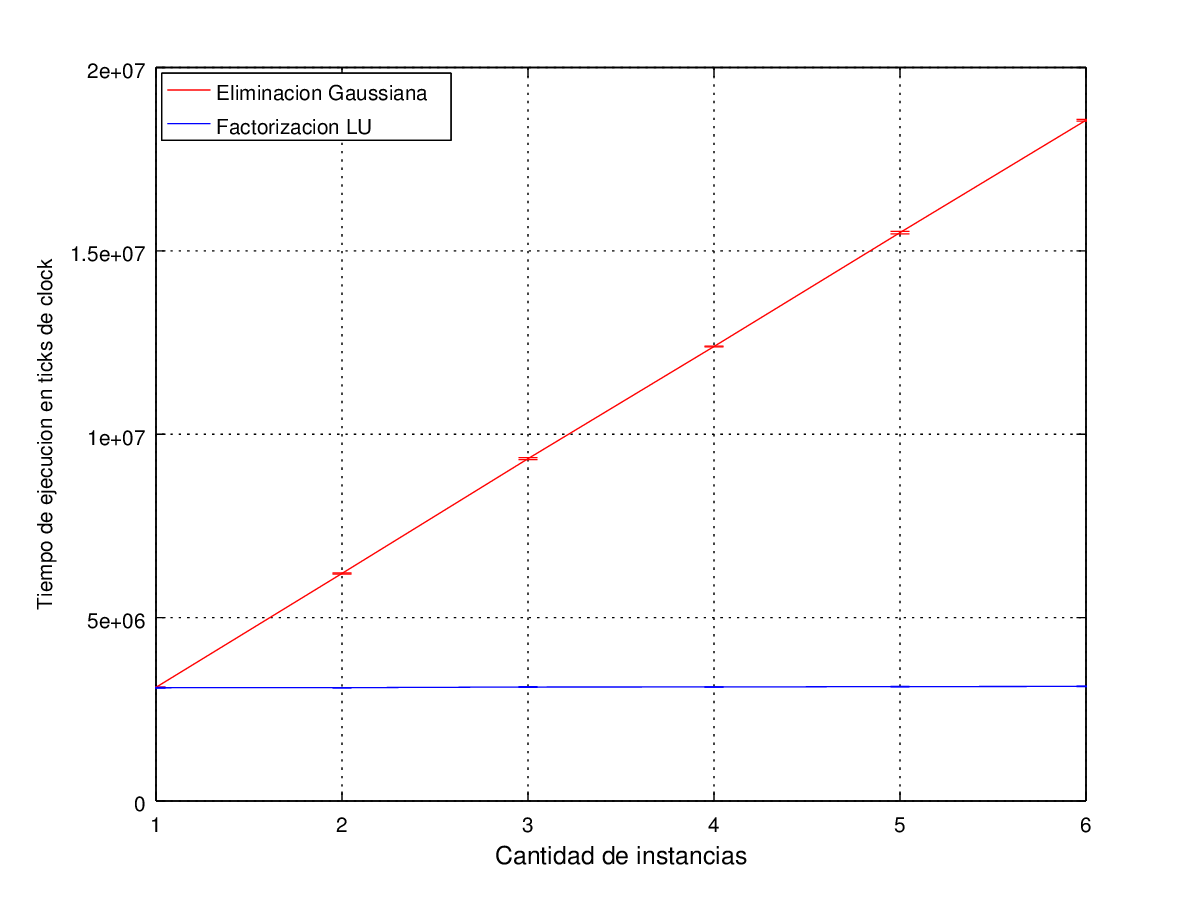
\includegraphics[width=9cm]{graficos/exp2/exp2.png} \\
          {\small Tiempo de ejecución en función del número de instancias del problema}
        \end{center}


      \subsubsection*{Discusión}
          Se observa que cuando hay pocas instancias, buscar la isoterma con el método de eliminación gaussiana o el de factorización LU es muy similar. 
          A medida que aumentan las instancias las diferencias entre ambos métodos aumentan, ya que la factorización LU se mantiene casi inmutable al aumentar las instancias mientras que la eliminación gaussiana aumenta notoriamente. 
          Se puede observar que lo que tarda la eliminación gaussiana cuando tiene 2 instancias es aproximadamente el doble de lo que tarda cuando es una única instancia. Cuando son 3 instancias, tarda el triple de lo que tarda cuando es una única instancia. 
          Sean $n$ instancias entonces lo que tarda la eliminación gaussiana es lo que tarda cuando es una única instancia $n$ veces. Esto es así ya que en este método numérico, para cada una de las instancias recalcula toda la matriz. En cambio la factorización LU, calcula la matriz una única vez.


    \subsubsection*{Experimento 3: Isoterma según temperatura en pared externa} 
      
      \subsubsection*{Presentación}
        En este experimento vamos a observar como varia la isoterma cuando modificamos la temperatura de la pared externa del horno. Para ello tomamos dos sistemas con temperaturas externas constantes pero distintos entre si. Graficamos para cada uno de ellos la isoterma 500. 
      
      \subsubsection*{Datos}
        Se evaluaron dos escenarios de prueba, ambos con los siguientes parámetros: $r_i = 30$, $r_e = 60$, $m+1 = 30$, $n = 30$, $T_i = 1500$, $iso = 500$. Se utilizaron temperaturas externas constantes en todos los puntos $(r_e, \theta)$ de la discretización, con $T_e(\theta) = 50$ grados en uno de los casos y $T_e(\theta) = 200$ grados en el otro. Se puede encontrar en los archivos adjuntos llamados exp3-$T_e(\theta)$.in la instancia pasada por parámetro.

      \subsubsection*{Hipótesis}
        Suponemos que cuando mayor sea la temperatura, la isoterma estará mas cerca de la pared externa del alto horno. 

      \subsubsection*{Resultados}
        En el gráfico puede observarse la ubicación estimada de la isoterma para cada uno de los casos, en magenta para $T_e(\theta) = 50${\degree}C (Isoterma A) y en verde para $T_e(\theta) = 200${\degree}C (Isoterma B).
        
            \begin{center}
              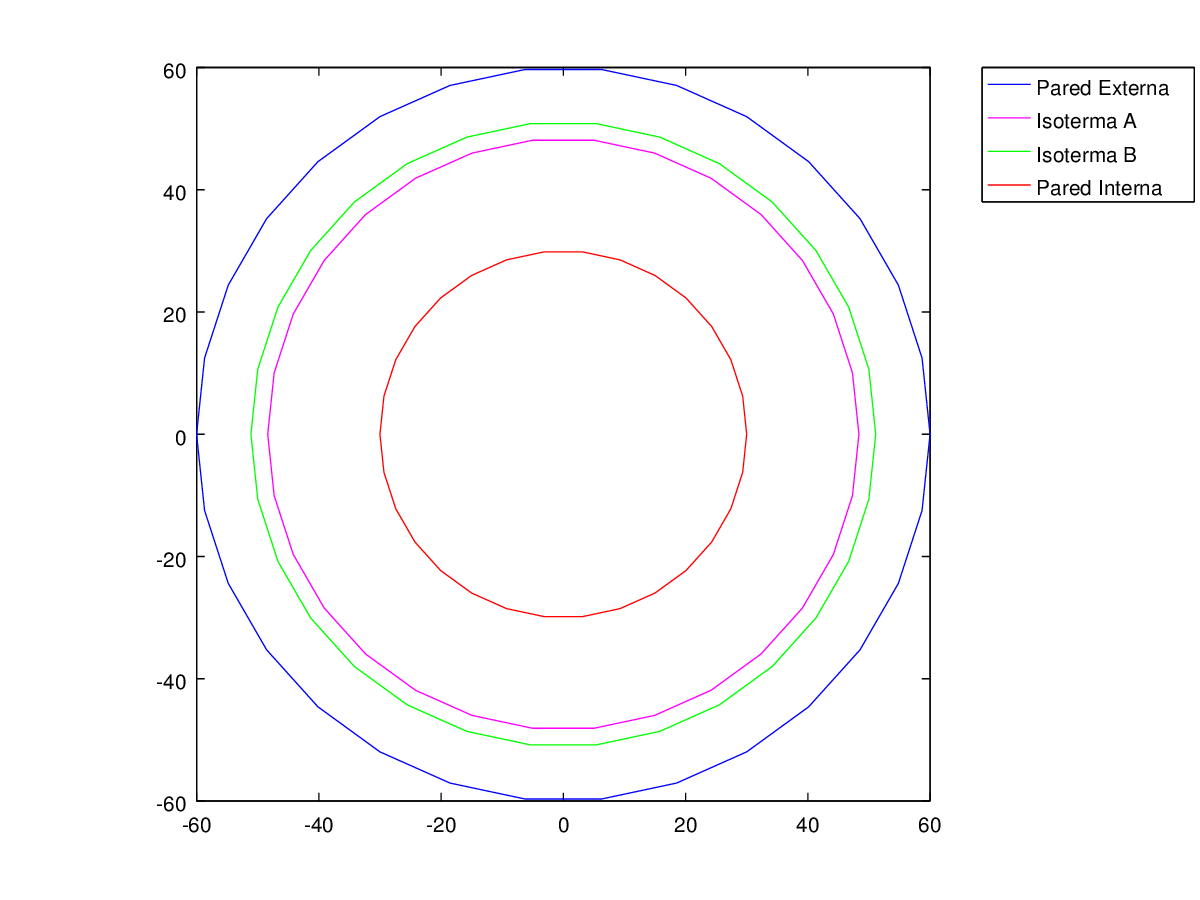
\includegraphics[width=9cm]{graficos/exp3/exp3.png} \\
              {\small Posiciones de las isotermas de 500{\degree}C}
            \end{center}

      \subsubsection*{Discusión}
        En este experimento se puede ver que la isoterma magenta se encuentra mas próxima a la pared interna del horno ya que corresponde a la instancia que tiene menor temperatura en la pared externa (50 grados). Lo mismo ocurre con la isoterma verde que se encuentra más cerca de la pared externa debido a que las temperaturas son más altas (200 grados).

        Además, en uno de los casos la temperatura externa es la máxima posible y en el otro la mínima. Podemos observar que nunca, con esta discretización, para ningún valor de temperaturas externas válidas, la isoterma puede pasar mas cerca de la pared externa del alto horno que lo que pasa la isoterma marcada en el gráfico con verde. Tampoco es posible que la isoterma pase más cerca de la pared interna del horno de lo que pasa la isoterma marcada en el gráfico con color magenta.


    \subsubsection*{Experimento 4: Isoterma según granularidad} 
      
      \subsubsection*{Presentación}
        Para realizar este experimento, se calcula la isoterma en un sistema donde la temperatura de la pared externa es constante, y la granularidad es muy alta. Llamaremos a esta, la isoterma de contraste. Se planea observar como varía la isoterma cuando se disminuye esta granularidad modificando únicamente la cantidad de radios a tener en cuenta (sin cambiar los ángulos), o modificando la cantidad de ángulos (sin cambiar los radios).
        Luego, se repite este proceso pero variando los valores de las temperaturas de la pared externa del horno. Esto valores son generados utilizando la función seno.

      \subsubsection*{Datos}

      \paragraph{Temperaturas constantes}

        Para ambos casos se consideraron instancias de prueba con los siguientes parámetros: $r_i = 30$, $r_e = 60$, $T_i = 1500$, $iso = 500$. Se utilizó una temperatura externa constante en todos los puntos $(r_e, \theta)$ de la discretización, ($T_e(\theta) = 50$). 

        En primer lugar, se calculó la solución del sistema y la posición estimada de la isoterma para una discretización considerablemente granular, con $m + 1 = 70$ y $n = 90$, para utilizar como caso de contraste. Reproducimos los gráficos que representan las temperaturas calculadas para todos los puntos de la discretización y la ubicación estimada de la isoterma. 

        \paragraph{Caso A} Se mantuvo constante la cantidad de radios de la discretización $m + 1 = 70$, y se tomaron instancias con diferentes cantidades de ángulos, para $n = 3, 5, 8, 10, 30, 50, 70$. Los gráficos que incluimos representan los resultados obtenidos para $n = 5, 10, 50$, reflejando las temperaturas calculadas y la ubicación estimada de la isoterma (en verde), comparada con la obtenida para el caso de contraste (en magenta). Se puede encontrar en los archivos adjuntos llamados exp4-const-ang-$n$.in  la instancia pasada por parámetro.

        \paragraph{Caso B} Se mantuvo constante la cantidad de ángulos de la discretización $n = 90$, y se tomaron instancias con diferentes cantidades de radios, para $m + 1 = 3, 5, 8, 10, 30, 50$. Los gráficos que incluimos representan los resultados obtenidos para $m + 1 = 3, 8, 30$, reflejando las temperaturas calculadas y la ubicación estimada de la isoterma (en verde), comparada con la obtenida para el caso de contraste (en magenta). Se puede encontrar en los archivos adjuntos llamados exp4-const-rad-$n$.in  la instancia pasada por parámetro.

      \paragraph{Variando temperaturas}

        Para ambos casos se consideraron instancias de prueba con los siguientes parámetros: $r_i = 30$, $r_e = 60$, $T_i = 1500$, $iso = 500$. Se generó una instancia de prueba con una temperatura externa variable entre 50 y 200{\degree}C en todos los puntos $(r_e, \theta)$ de la discretización. 
        Para la generación de las instancias de prueba se consideró la función $T_e(\theta) = 125 + 75 \sin(2\theta)$ para que la variación de temperaturas sea suave.
        En primer lugar, se calculó la solución del sistema y la posición estimada de la isoterma para una discretización considerablemente granular, con $m + 1 = 70$ y $n = 90$, para utilizar como caso de contraste. Reproducimos los gráficos que representan las temperaturas calculadas para todos los puntos de la discretización y la ubicación estimada de la isoterma.

        \paragraph{Caso A} Se mantuvo constante la cantidad de radios de la discretización $m + 1 = 70$, y se tomaron instancias con diferentes cantidades de ángulos, para $n = 3, 5, 8, 10, 30, 50, 70$. Los gráficos que incluimos representan los resultados obtenidos para $n = 5, 10, 50$, reflejando las temperaturas calculadas y la ubicación estimada de la isoterma (en verde), comparada con la obtenida para el caso de contraste (en magenta). Se puede encontrar en los archivos adjuntos llamados exp4-seno-ang-$n$.in la instancia pasada por parámetro.
        
        \paragraph{Caso B} Se mantuvo constante la cantidad de ángulos de la discretización $n = 90$, y se tomaron instancias con diferentes cantidades de ángulos, para $m + 1 = 3, 5, 8, 10, 30, 50$. Los gráficos que incluimos representan los resultados obtenidos para $m + 1 = 3, 8, 30$, reflejando las temperaturas calculadas y la ubicación estimada de la isoterma (en verde), comparada con la obtenida para el caso de contraste (en magenta). Se puede encontrar en los archivos adjuntos llamados exp4-seno-rad-$n$.in la instancia pasada por parámetro.
     
      \subsubsection*{Hipótesis}
          Se espera que, en ambos casos, cuanto menor sea la granularidad de la discretización, más alejada estará la isoterma calculada de la de contraste. Si tomamos menos particiones sobre radios, la distancia entre ellos aumenta. Como el cálculo de la isoterma supone que la temperatura entre dos de ellos, uno más lejano y otro más cercano a la pared, decrece en forma lineal, lo cual podría generar que el error aumente. Si tomamos menos particiones sobre ángulos, existen puntos que no van a ser considerados en el cálculo de la isoterma, por lo tanto, el error también es mayor. 


      \subsubsection*{Resultados}

        Para estos gráficos tomaremos el color rojo como las temperaturas más calientes siendo el rojo más oscuro la temperatura de 1500 grados y azul las temperaturas más frías siendo el azul más oscuro 50 grados.
        
      \subsubsection*{Temperaturas constantes}

        {\centering \begin{tabular}{cc}
           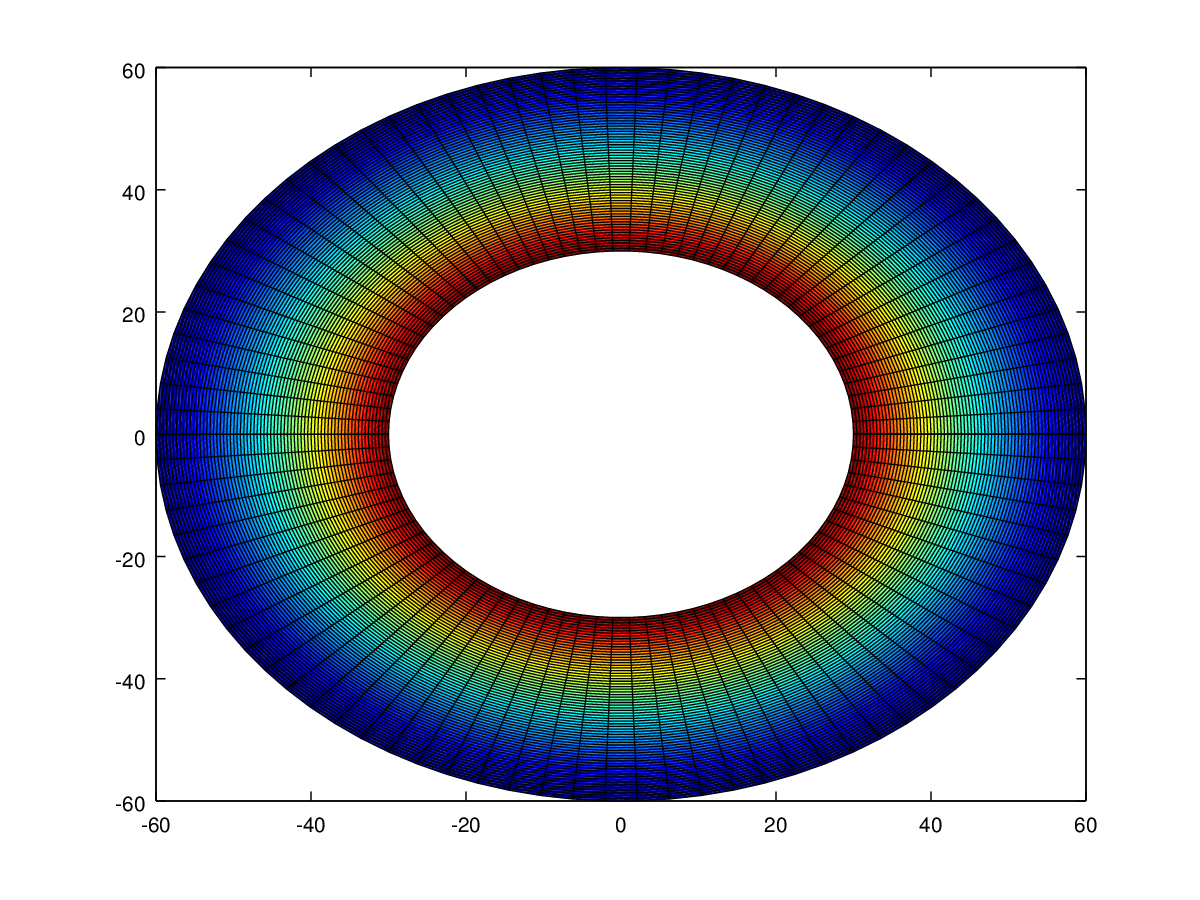
\includegraphics[height=5cm]{graficos/exp4/const/exp4-const-contraste.png} & 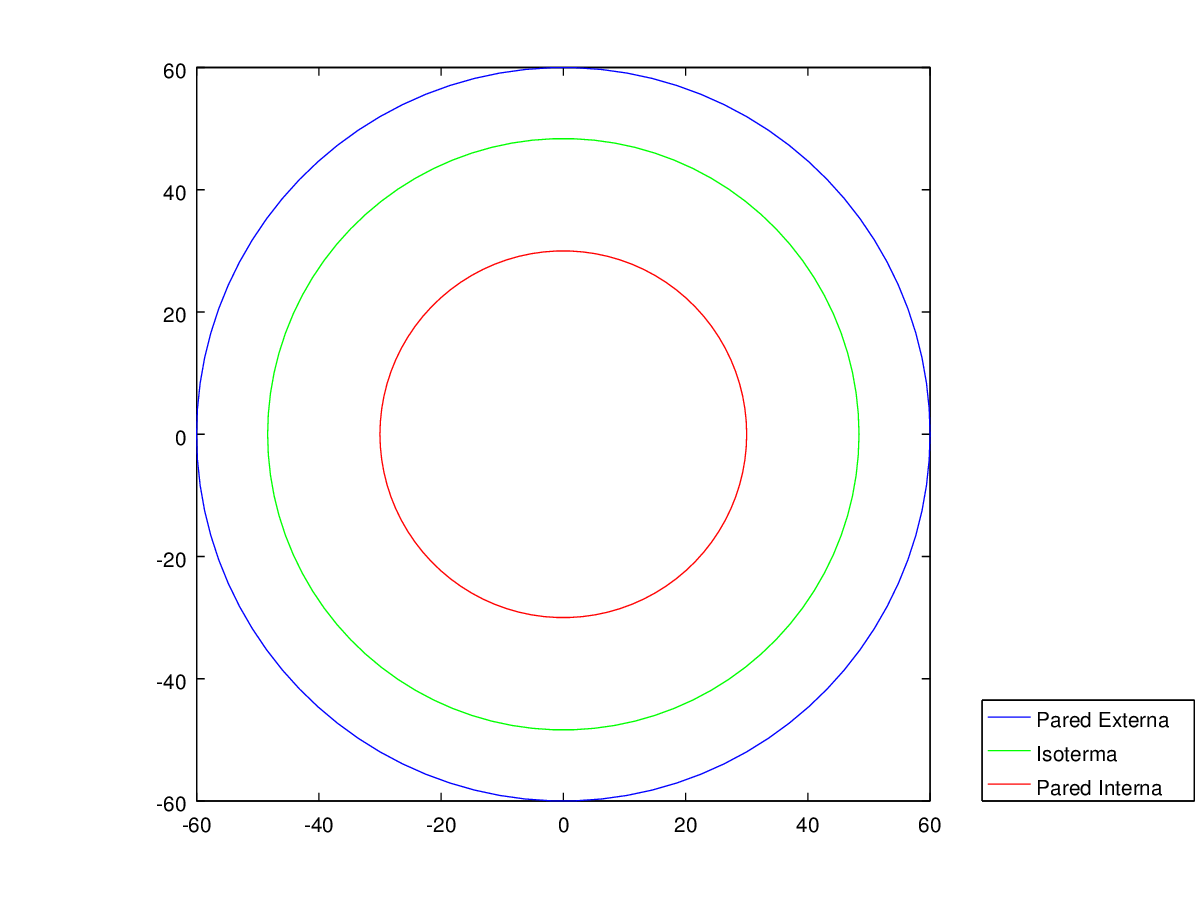
\includegraphics[height=5cm]{graficos/exp4/const/exp4-const-contraste-iso.png} \\
          {\small Temperaturas obtenidas} &
          {\small Posición estimada de la isoterma 500{\degree}C} \\
         \end{tabular}}

       \subsubsection*{Caso A}
         
          {\centering \begin{tabular}{ccc}
            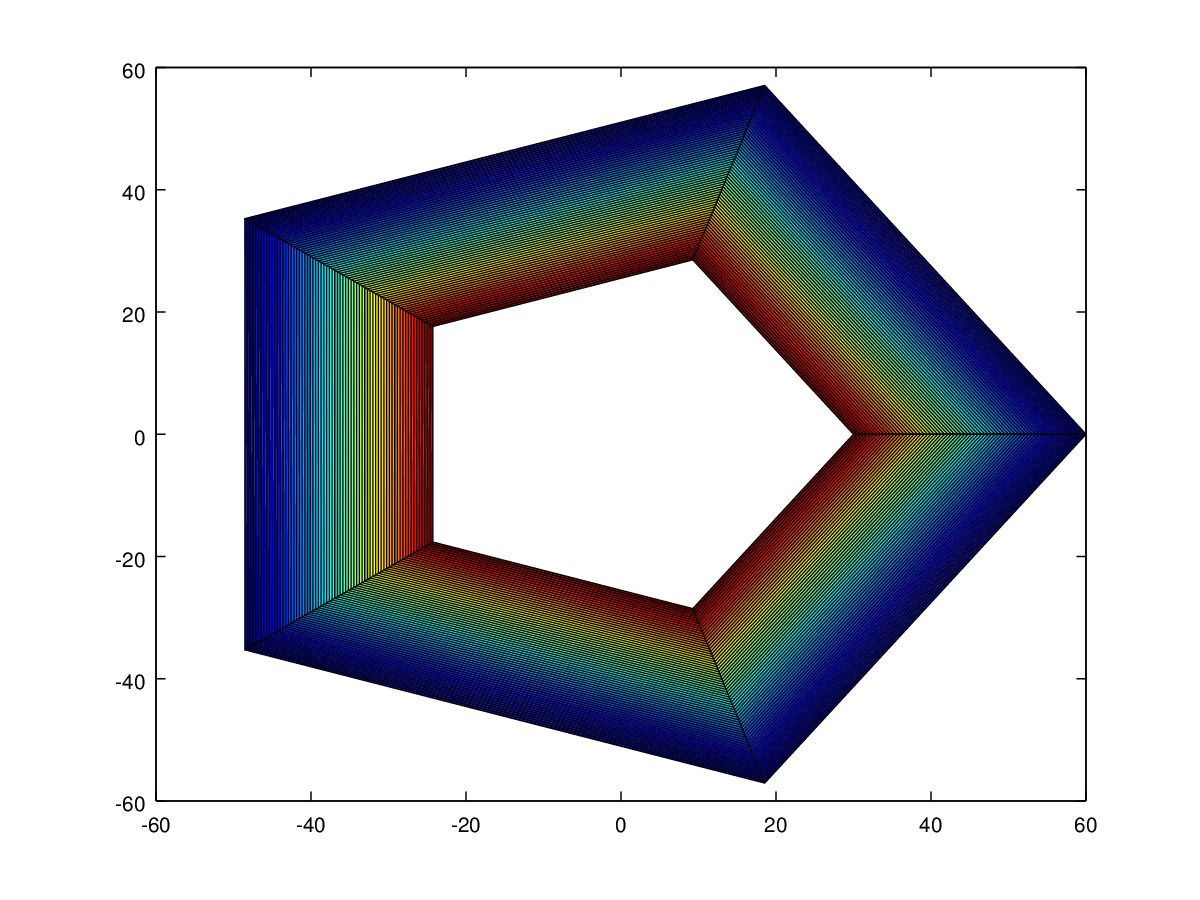
\includegraphics[width=4.5cm]{graficos/exp4/const/exp4-const-ang-5.png} &
            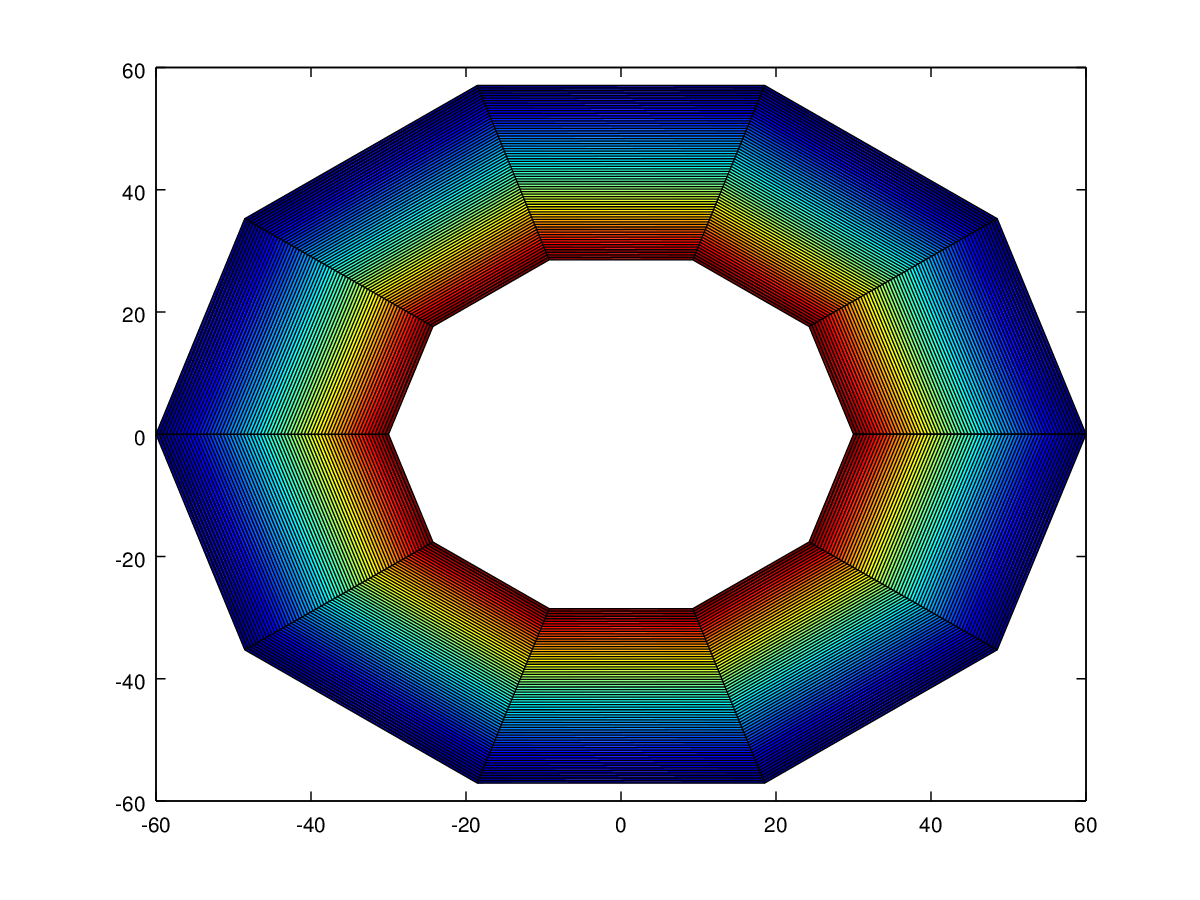
\includegraphics[width=4.5cm]{graficos/exp4/const/exp4-const-ang-10.png} &
            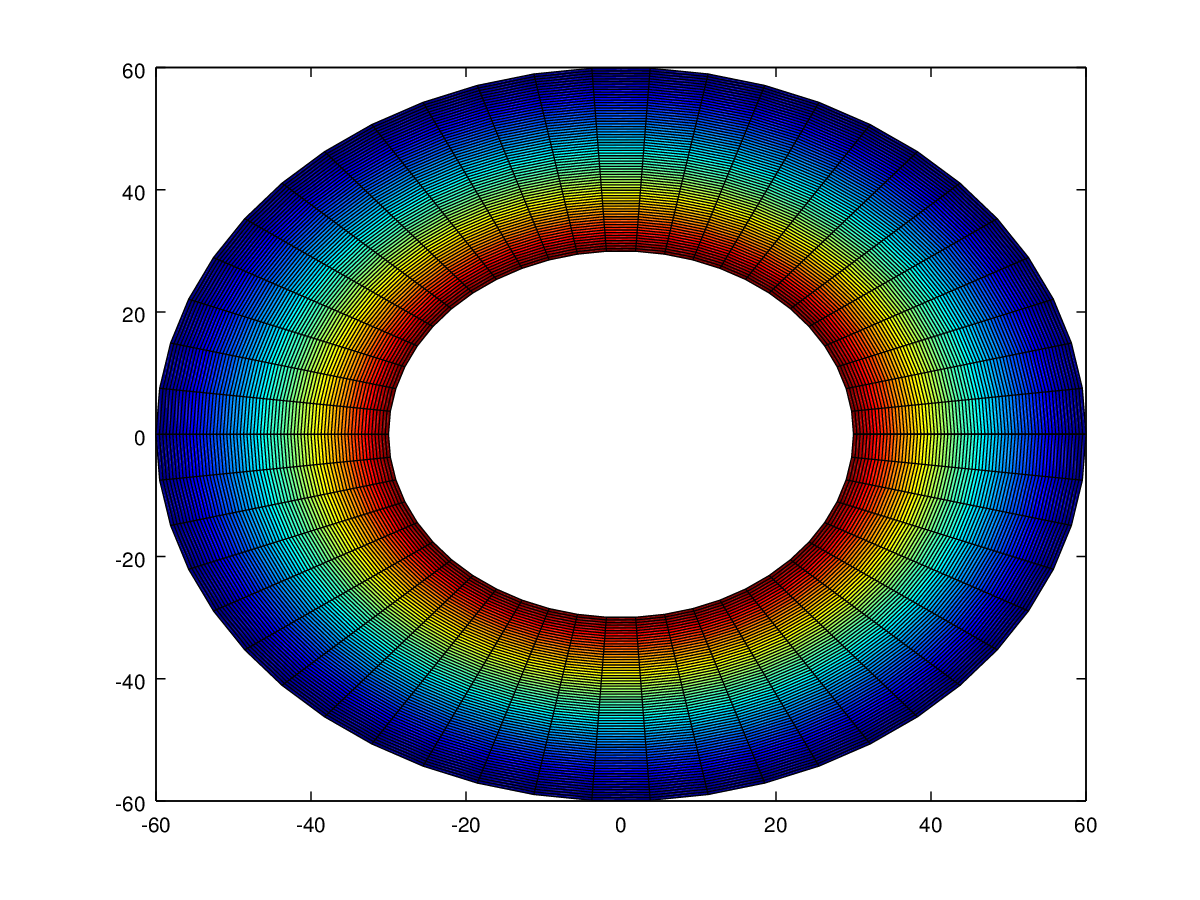
\includegraphics[width=4.5cm]{graficos/exp4/const/exp4-const-ang-50.png} \\
            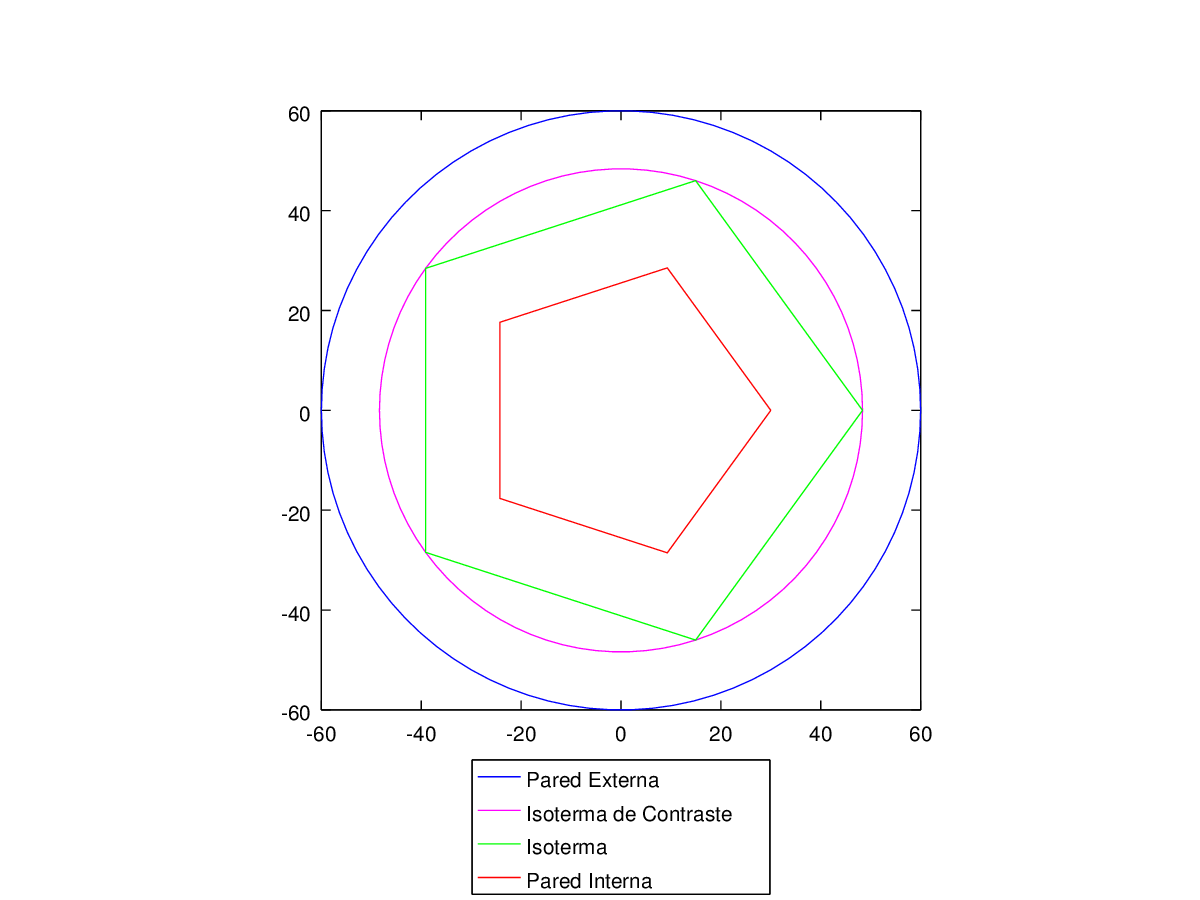
\includegraphics[width=5cm]{graficos/exp4/const/exp4-const-ang-5-iso.png} &
            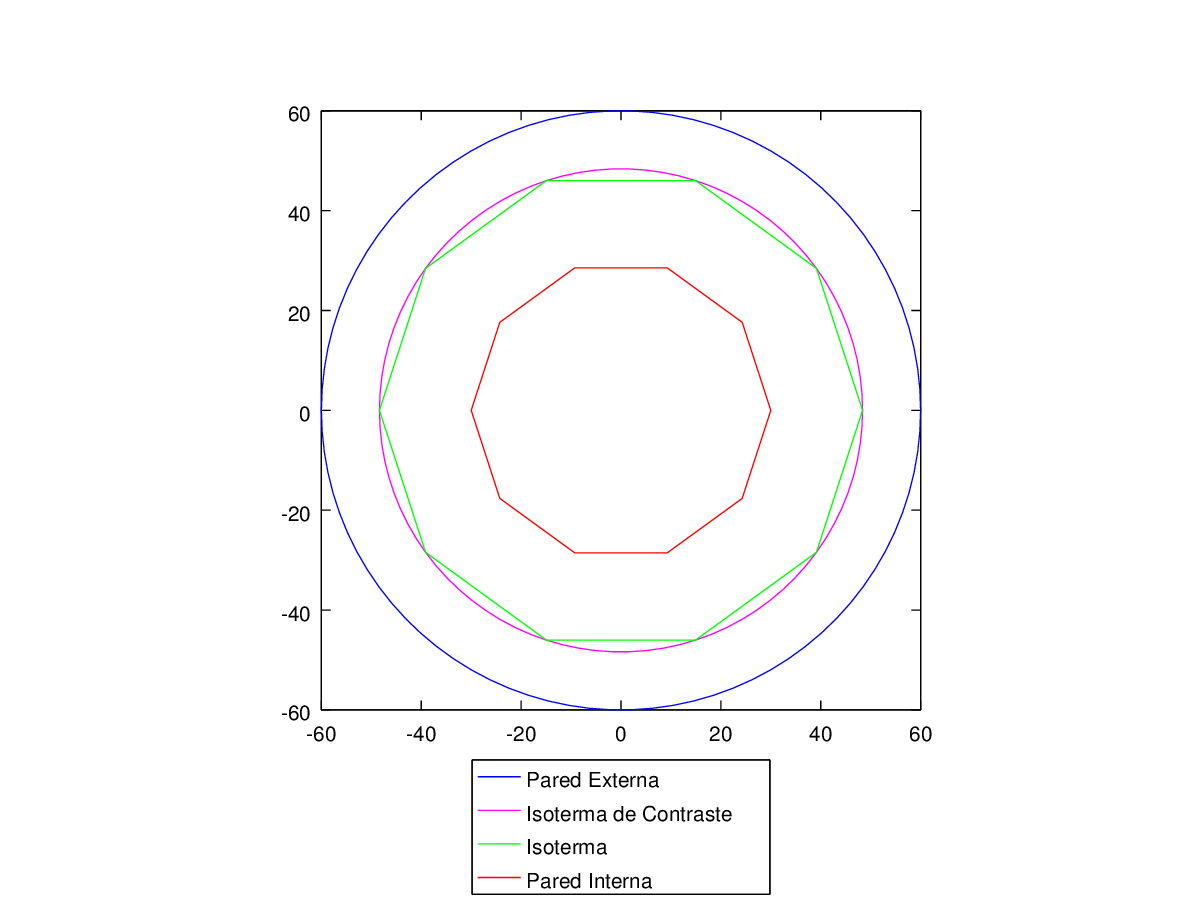
\includegraphics[width=5cm]{graficos/exp4/const/exp4-const-ang-10-iso.png} &
            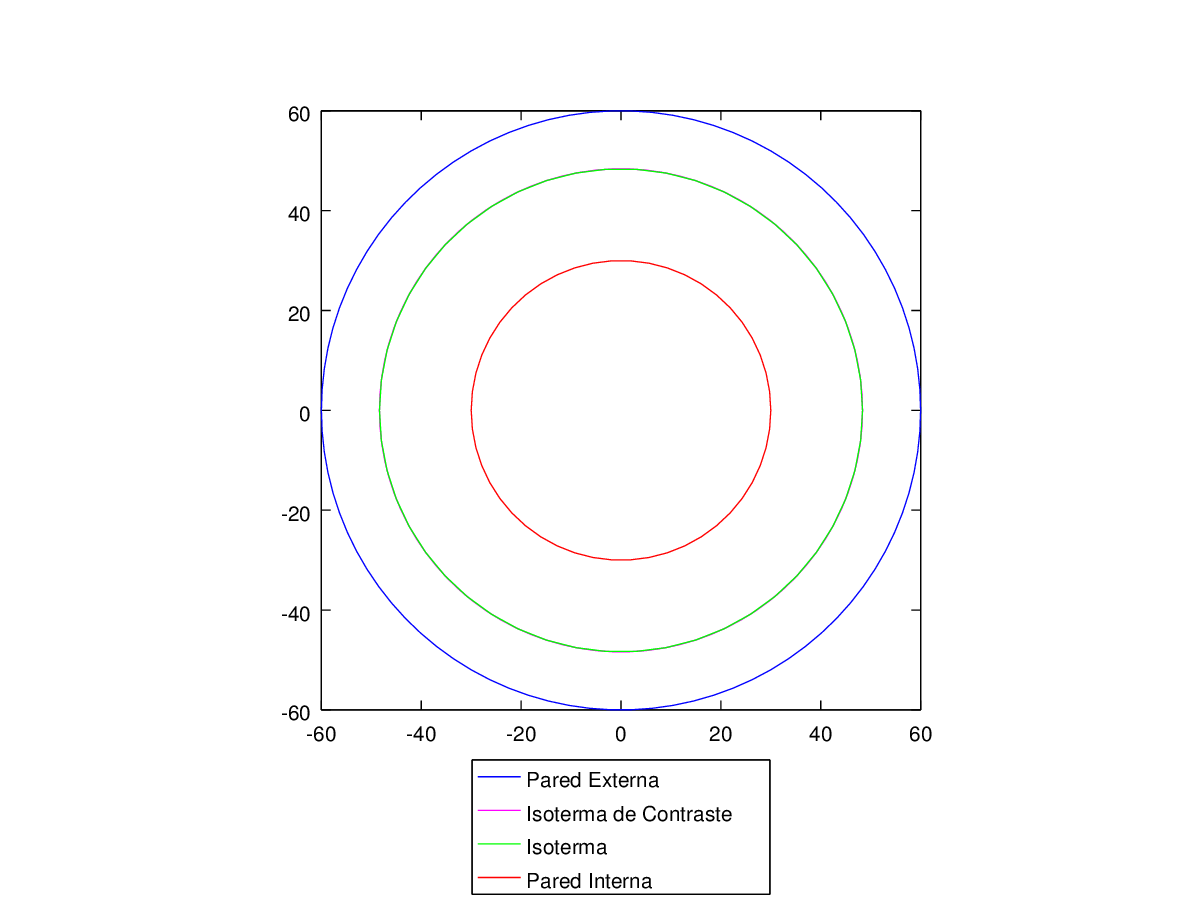
\includegraphics[width=5cm]{graficos/exp4/const/exp4-const-ang-50-iso.png} \\
            {\small $n = 5$} &
            {\small $n = 10$} &
            {\small $n = 50$} \\
          \end{tabular}}

      \subsubsection*{Caso B}
        
          {\centering \begin{tabular}{ccc}
            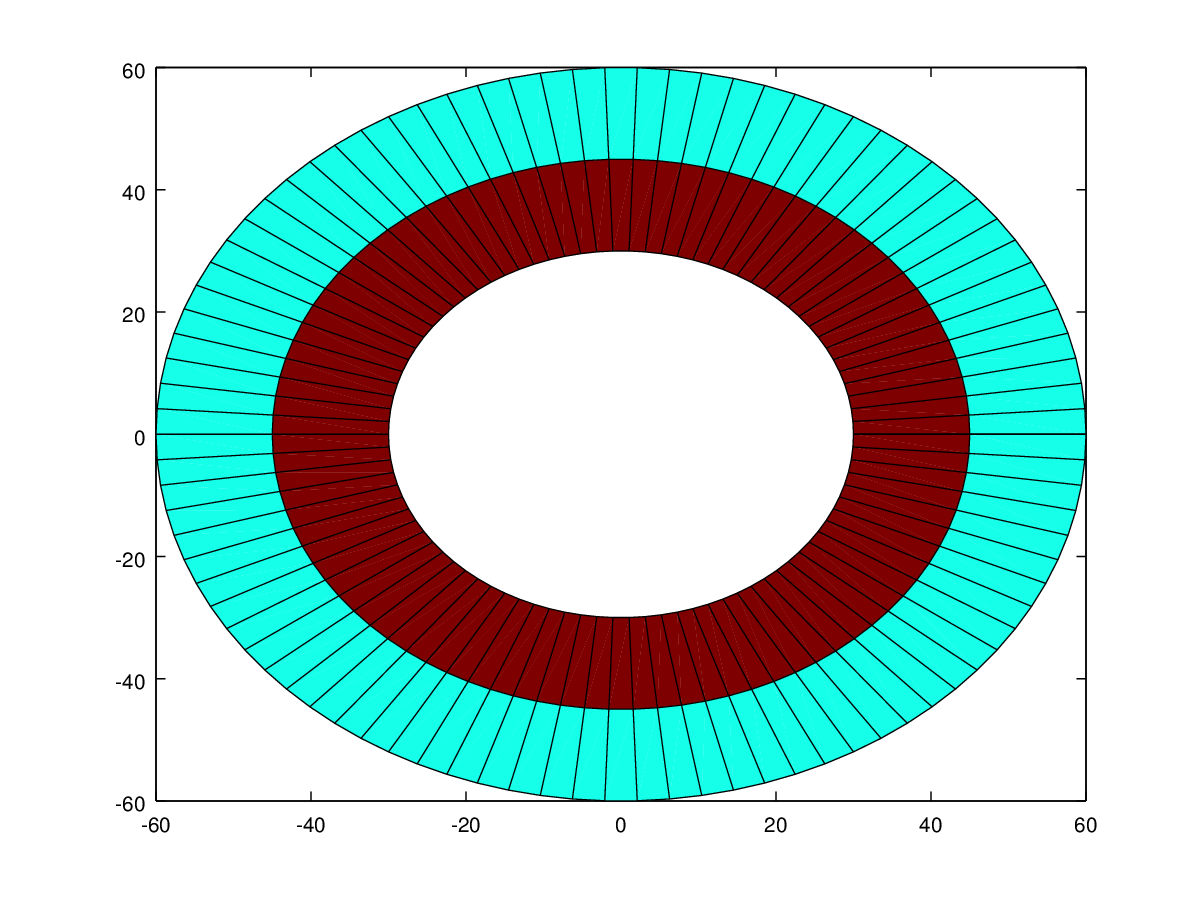
\includegraphics[width=4.5cm]{graficos/exp4/const/exp4-const-rad-3.png} &
            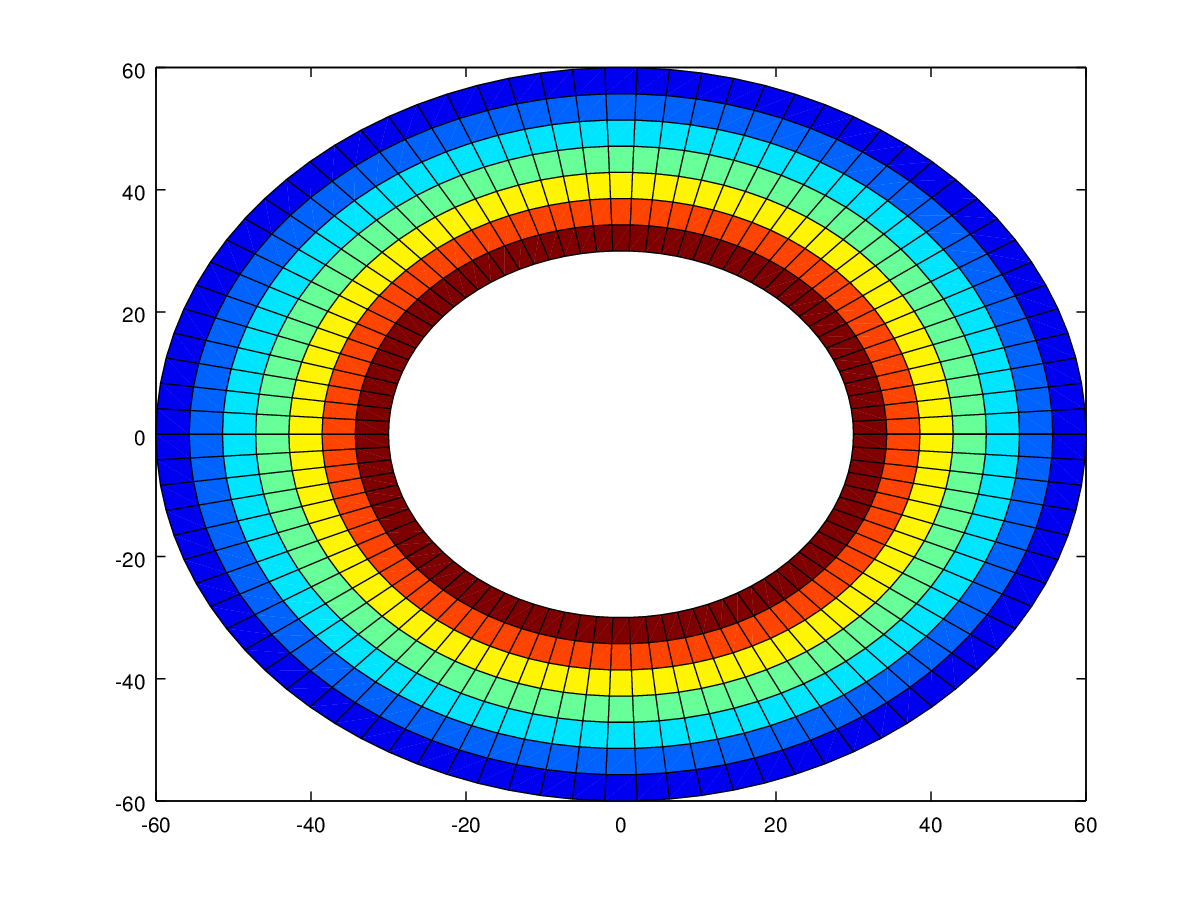
\includegraphics[width=4.5cm]{graficos/exp4/const/exp4-const-rad-8.png} &
            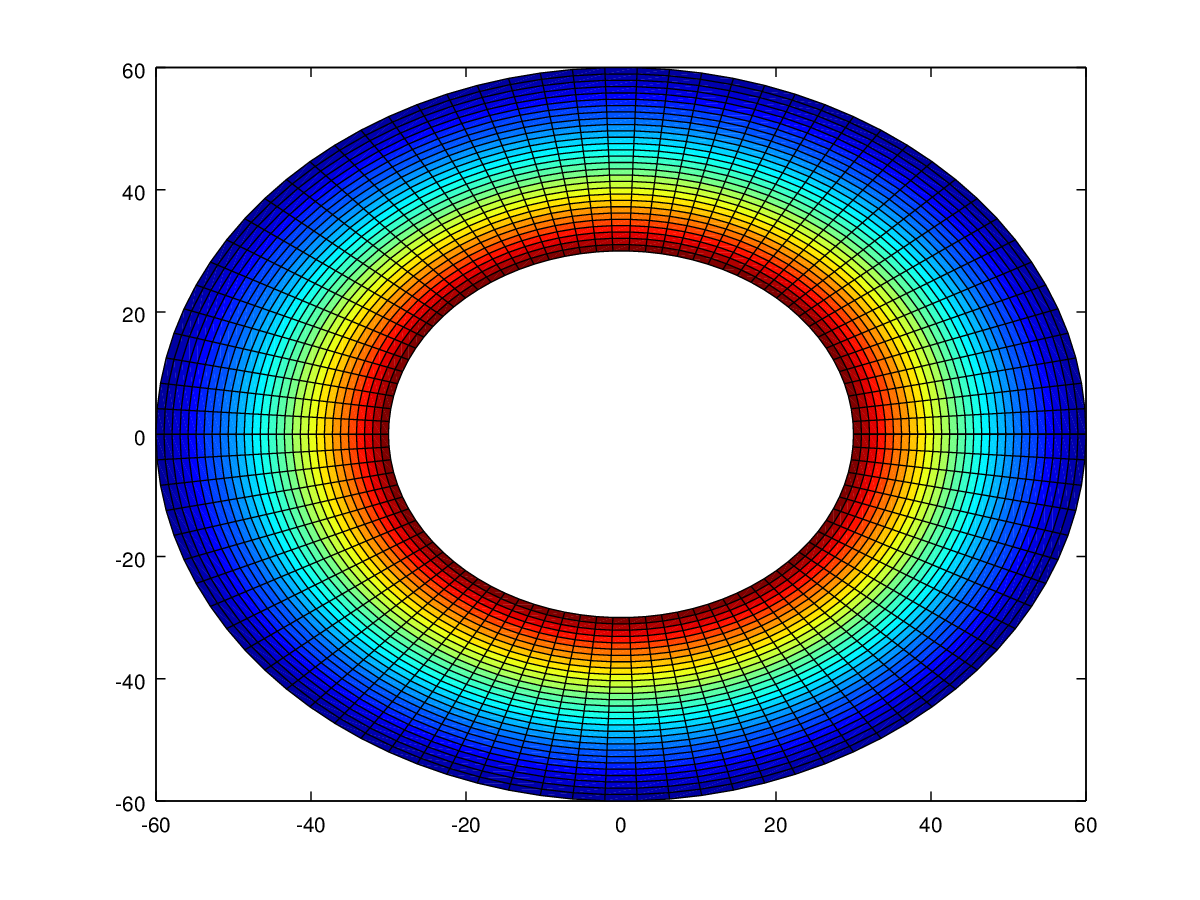
\includegraphics[width=4.5cm]{graficos/exp4/const/exp4-const-rad-30.png} \\
            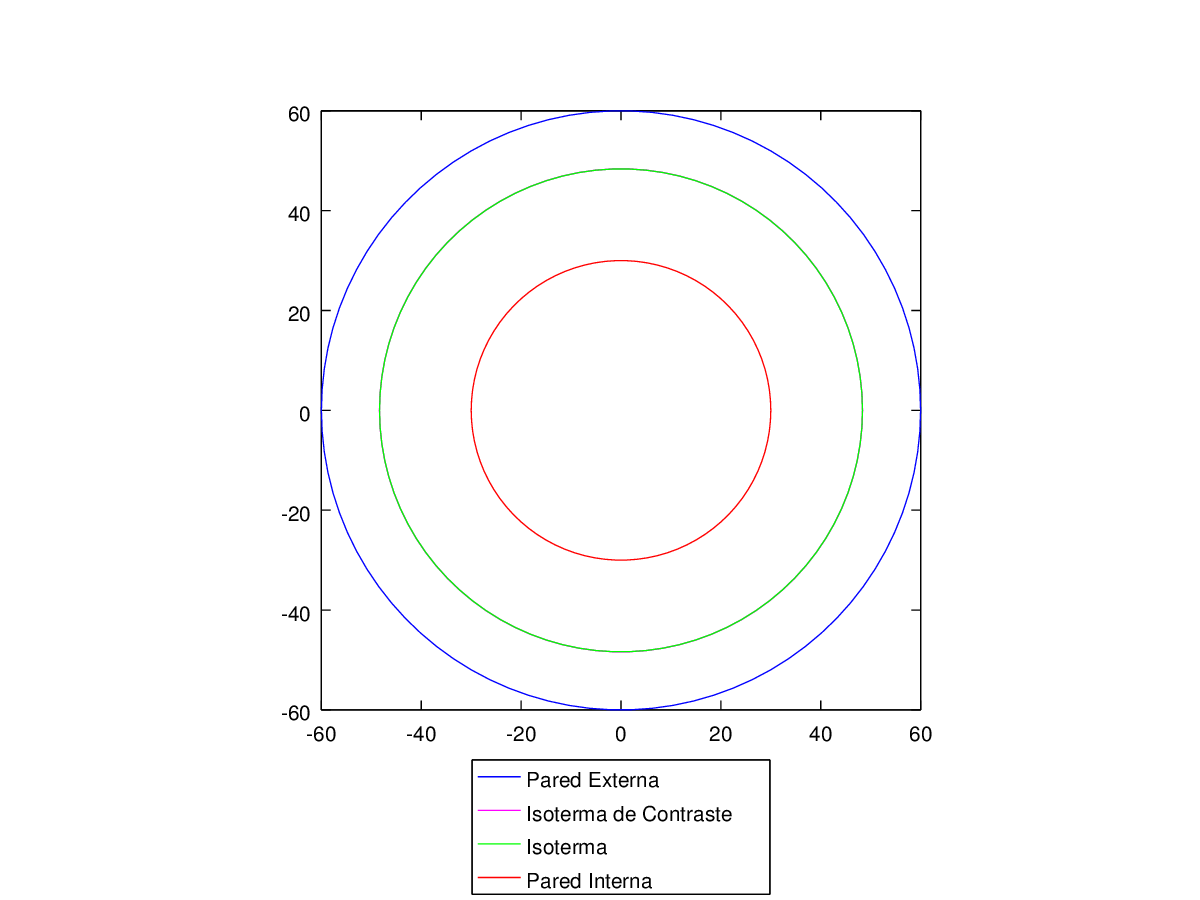
\includegraphics[width=5cm]{graficos/exp4/const/exp4-const-rad-3-iso.png} &
            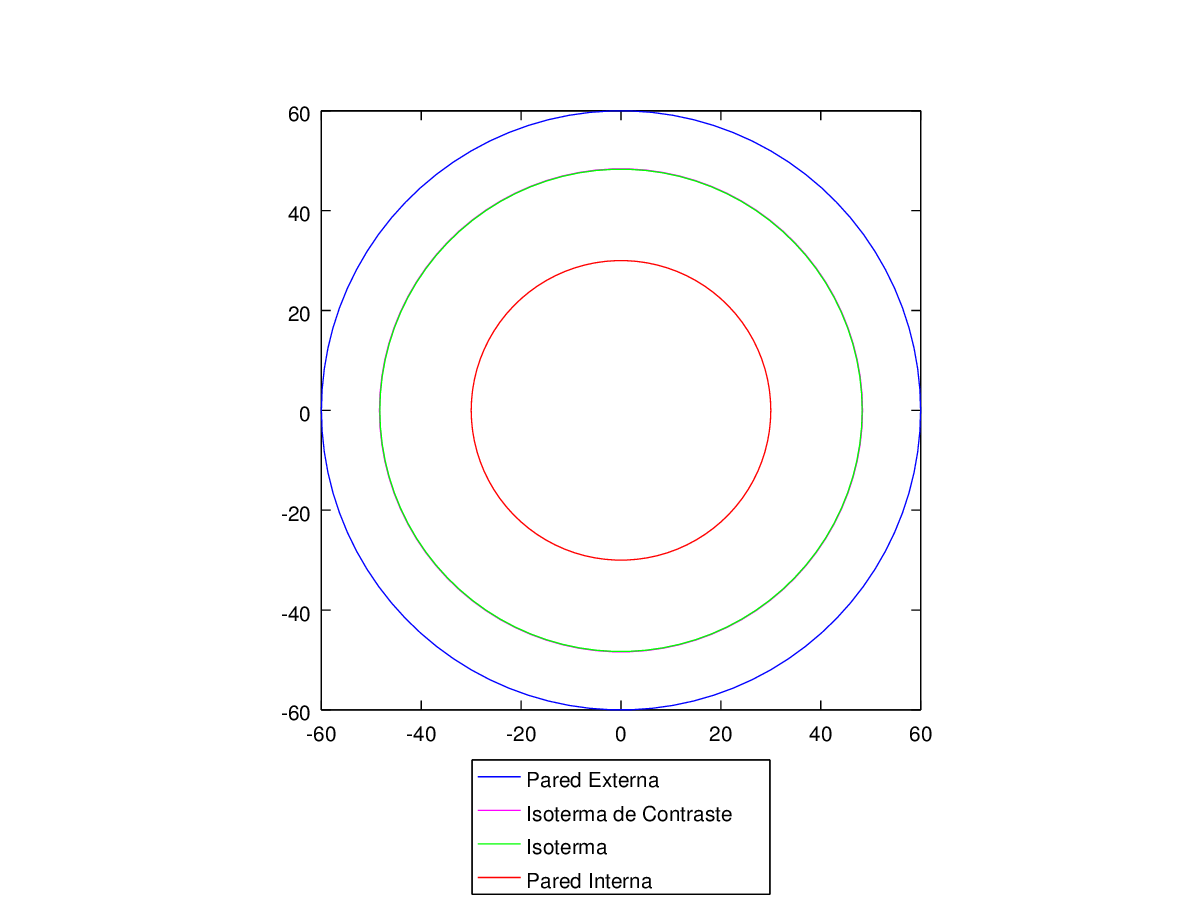
\includegraphics[width=5cm]{graficos/exp4/const/exp4-const-rad-8-iso.png} &
            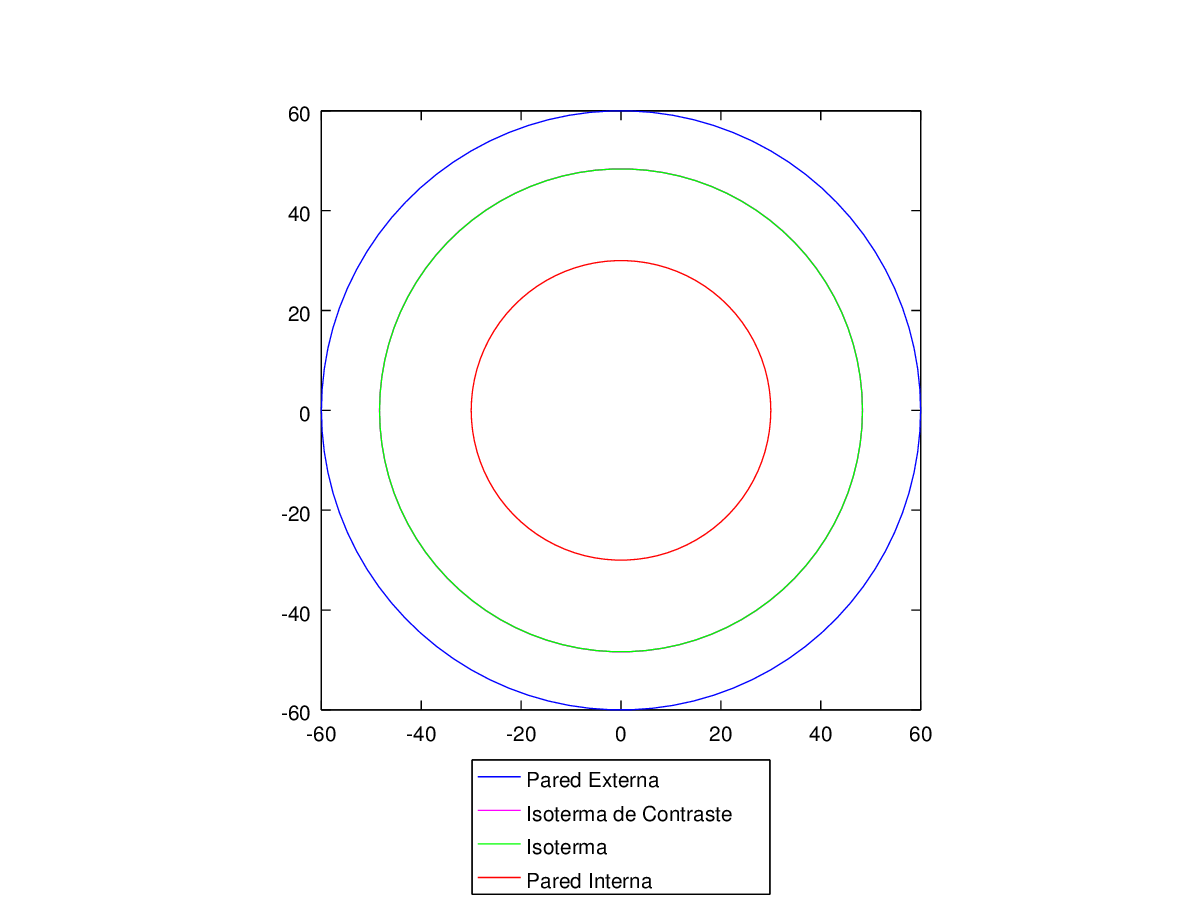
\includegraphics[width=5cm]{graficos/exp4/const/exp4-const-rad-30-iso.png} \\
            {\small $m+1 = 3$} &
            {\small $m+1 = 8$} &
            {\small $m+1 = 30$} \\
          \end{tabular}}

      \subsubsection*{Variando temperaturas}

        {\centering \begin{tabular}{cc}
          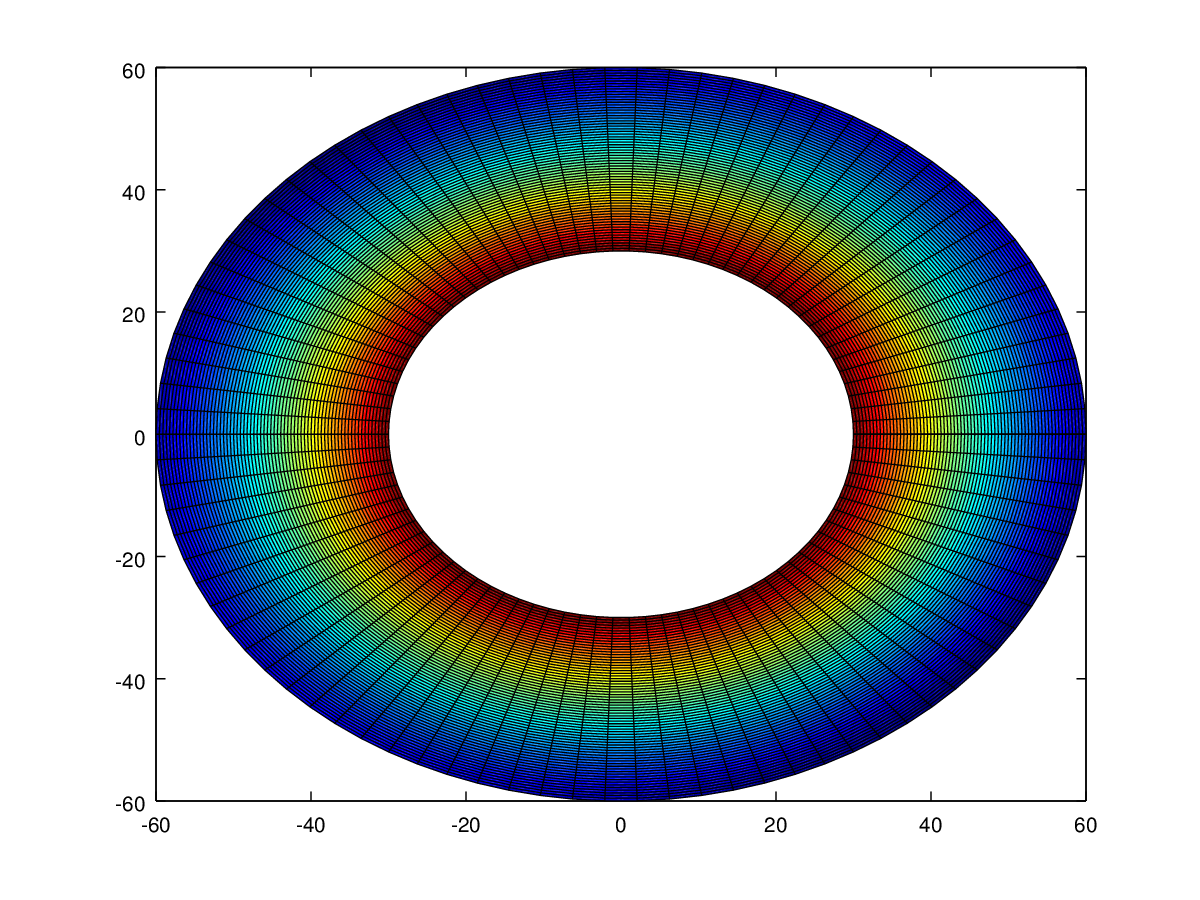
\includegraphics[height=5cm]{graficos/exp4/seno/exp4-seno-contraste.png} & 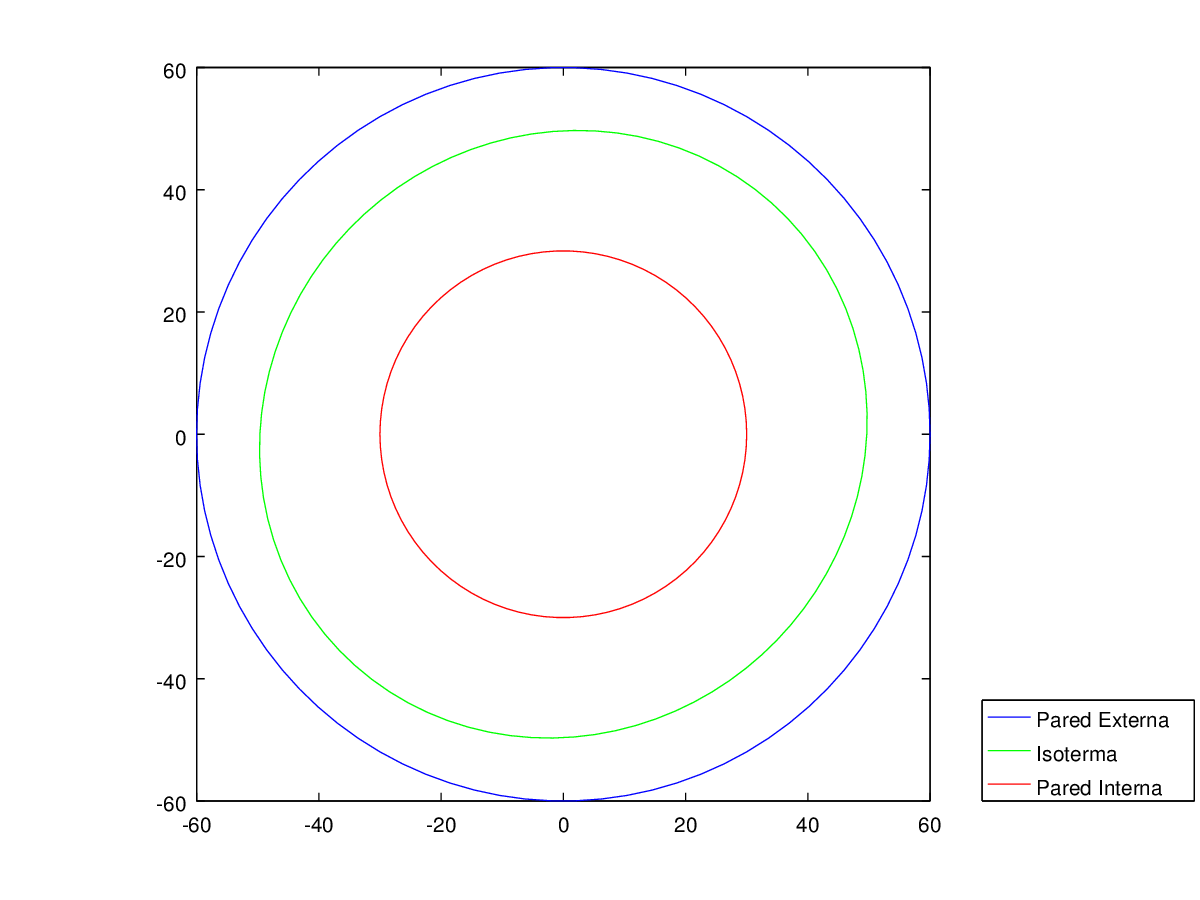
\includegraphics[height=5cm]{graficos/exp4/seno/exp4-seno-contraste-iso.png} \\
          {\small Temperaturas obtenidas} &
          {\small Posición estimada de la isoterma 500{\degree}C} \\
        \end{tabular}}

        \subsubsection*{Caso A}
            {\centering \begin{tabular}{ccc}
              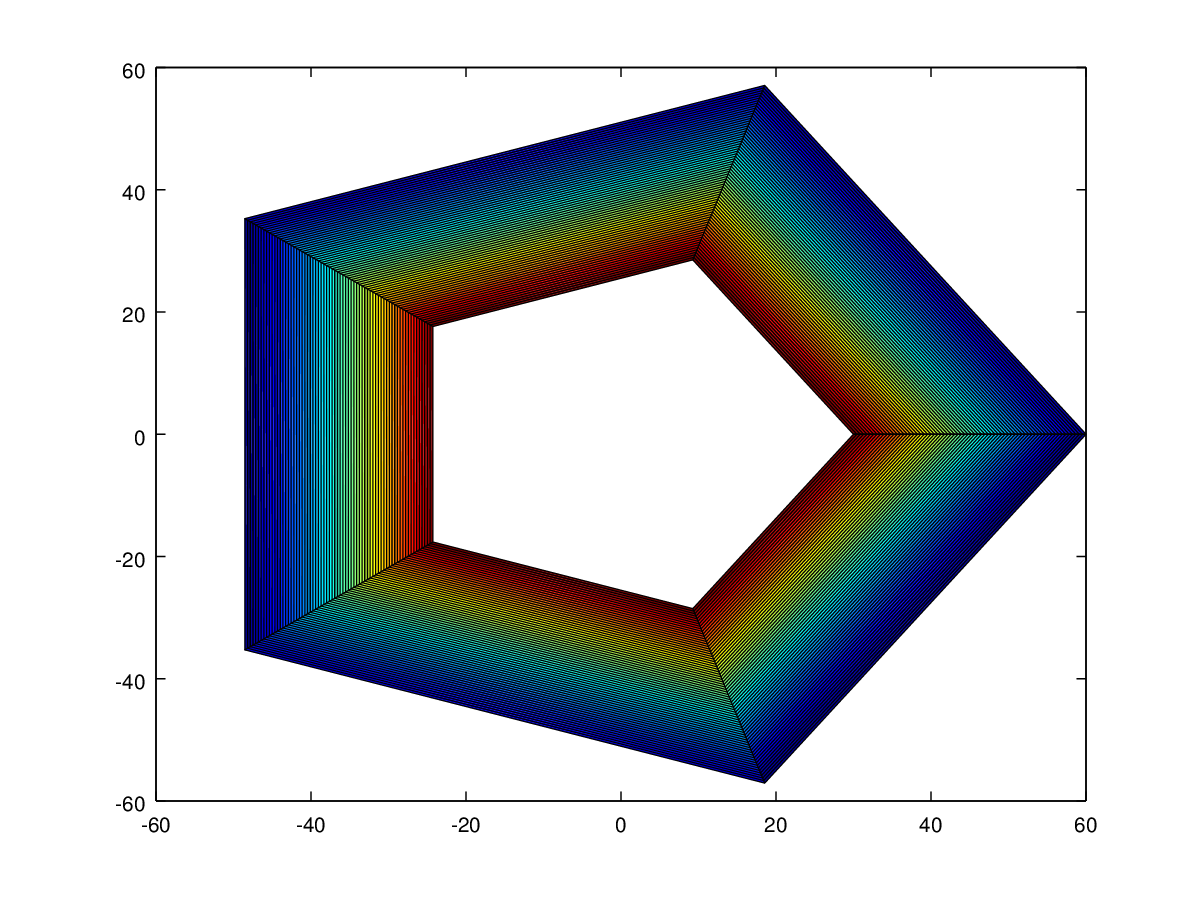
\includegraphics[width=4.5cm]{graficos/exp4/seno/exp4-seno-ang-5.png} &
              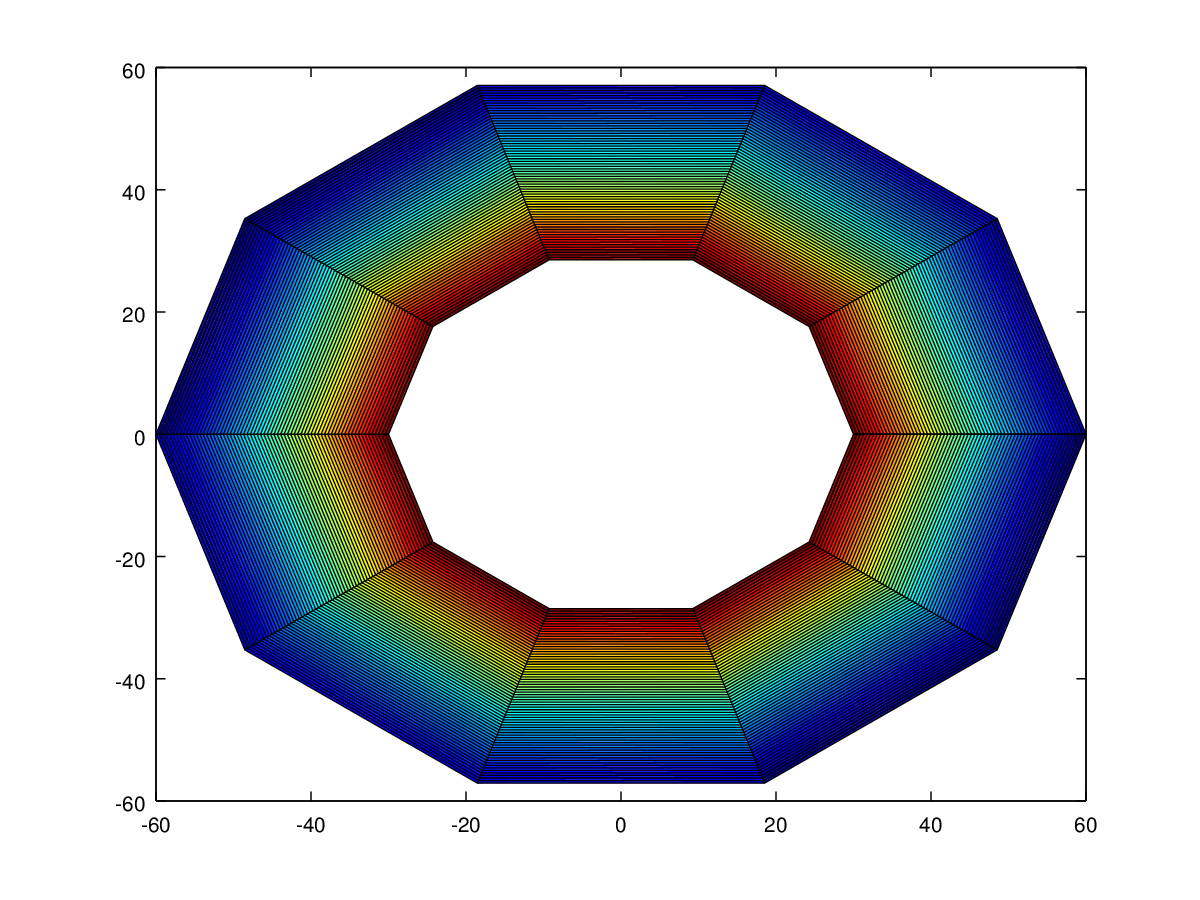
\includegraphics[width=4.5cm]{graficos/exp4/seno/exp4-seno-ang-10.png} &
              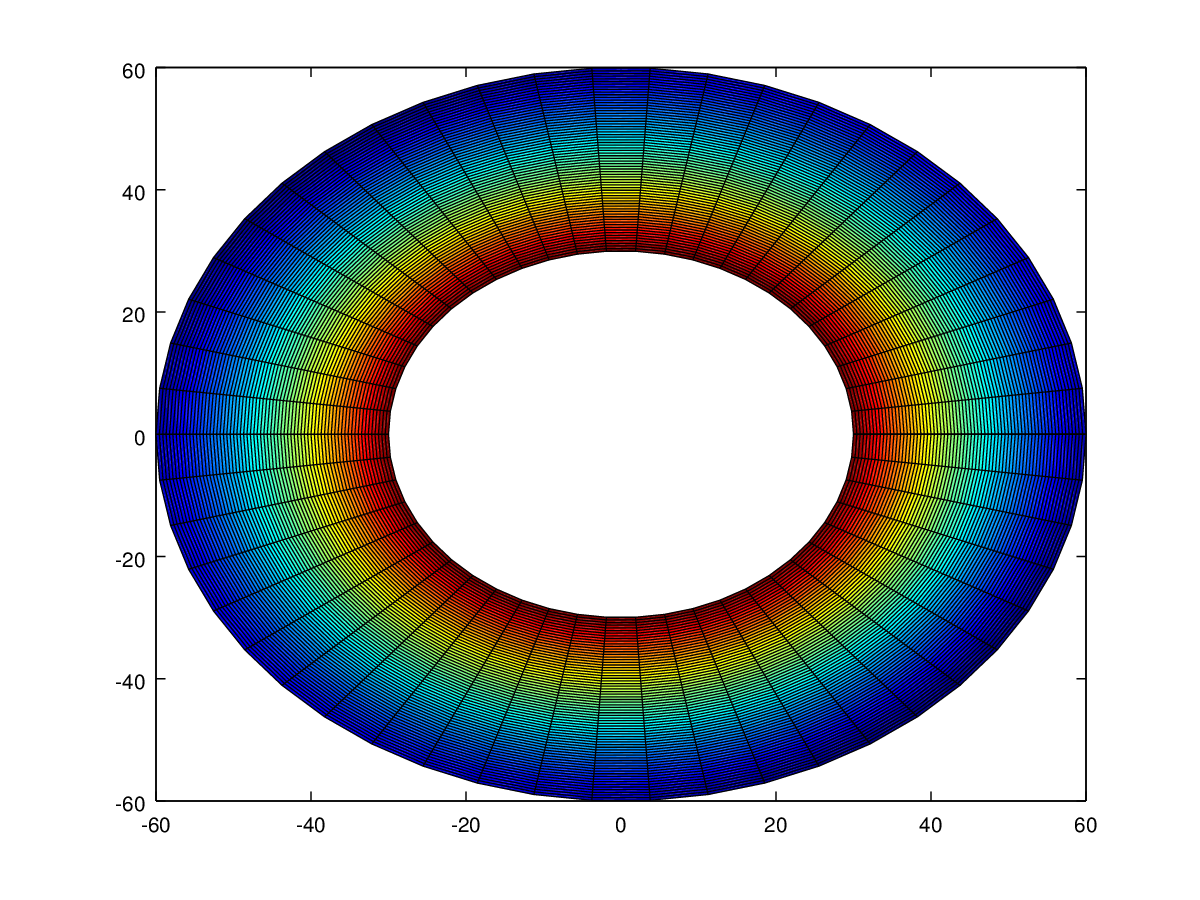
\includegraphics[width=4.5cm]{graficos/exp4/seno/exp4-seno-ang-50.png} \\
              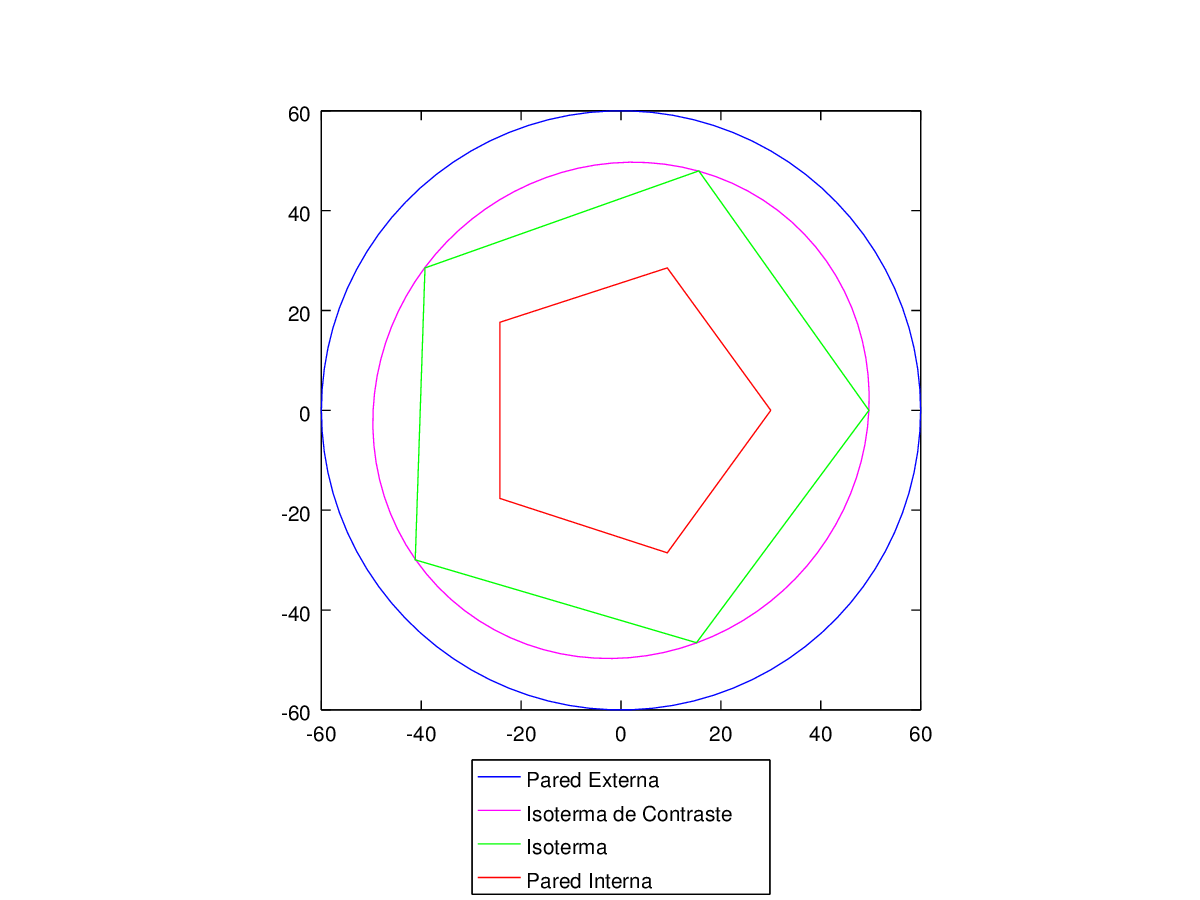
\includegraphics[width=5cm]{graficos/exp4/seno/exp4-seno-ang-5-iso.png} &
              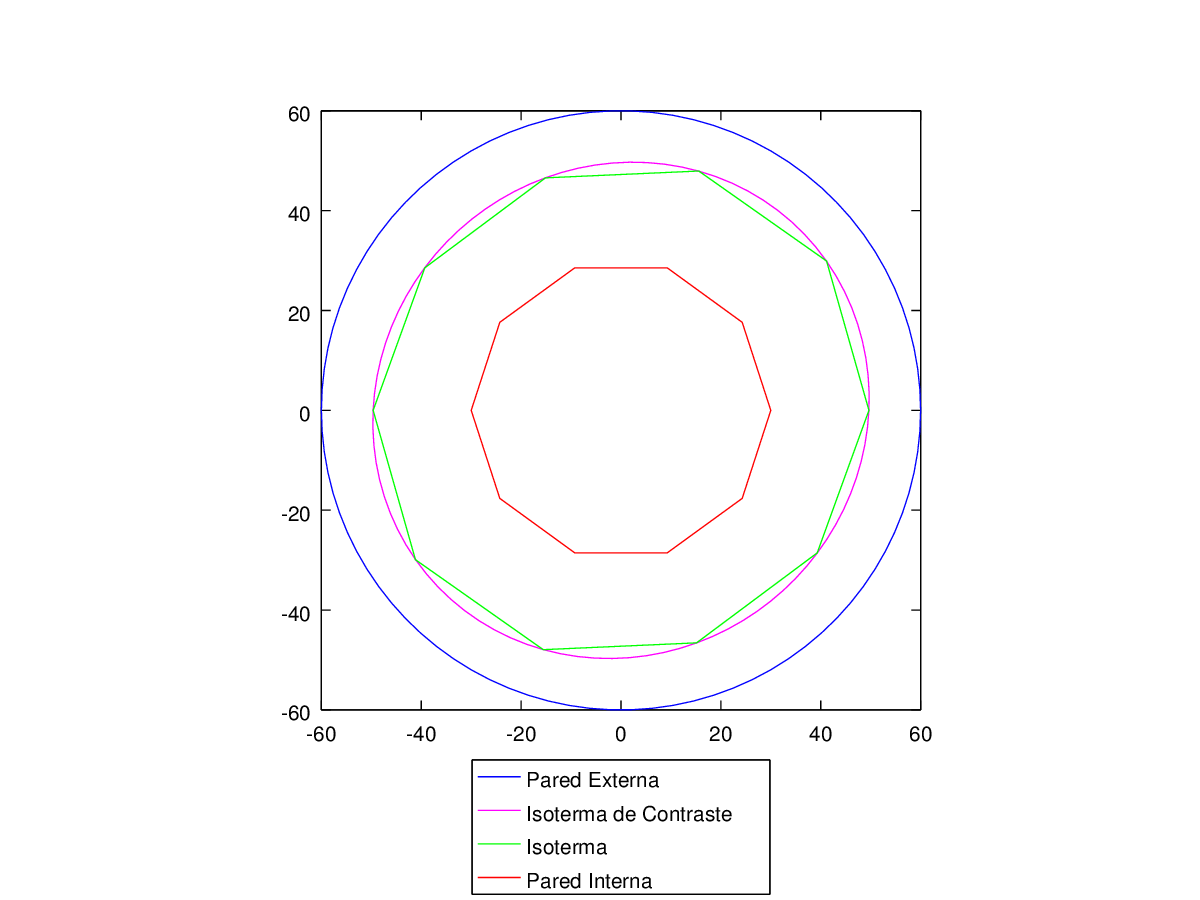
\includegraphics[width=5cm]{graficos/exp4/seno/exp4-seno-ang-10-iso.png} &
              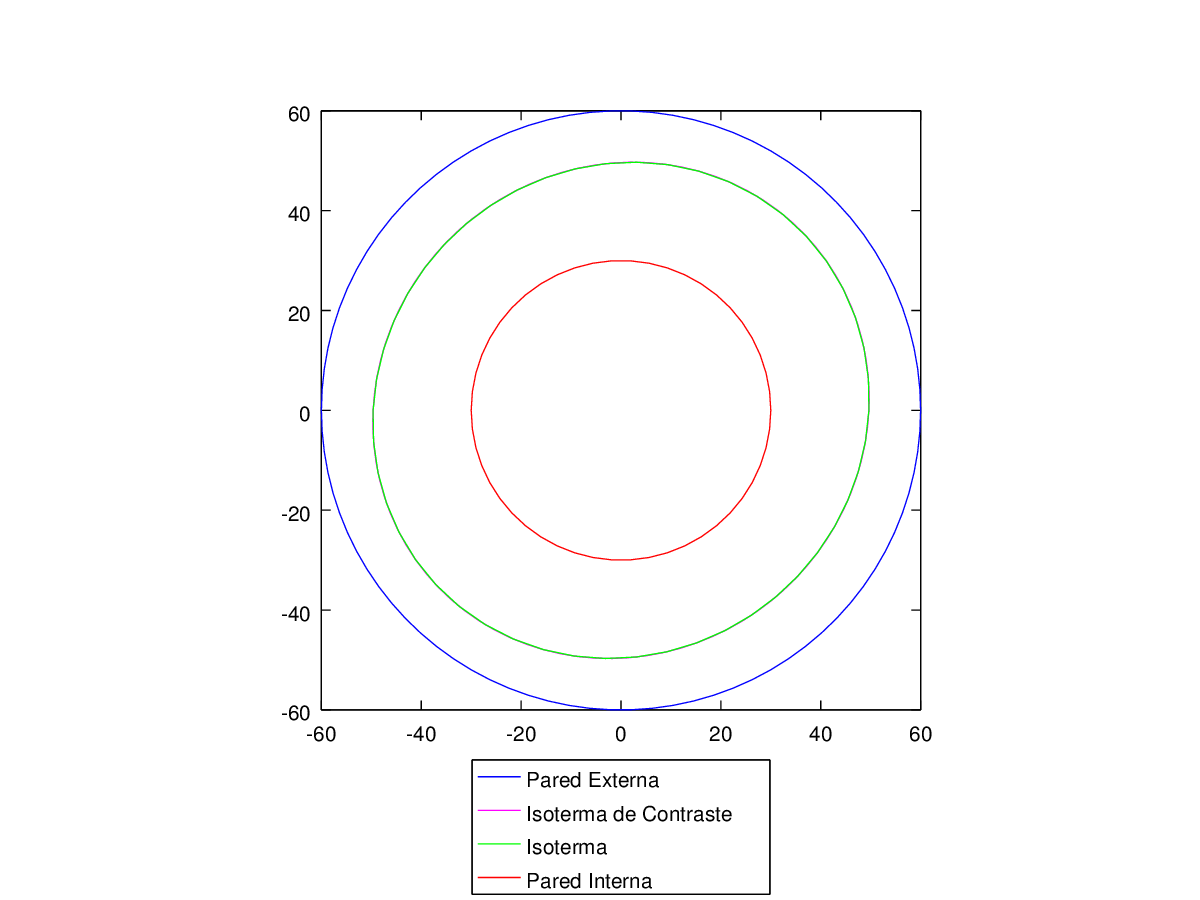
\includegraphics[width=5cm]{graficos/exp4/seno/exp4-seno-ang-50-iso.png} \\
              {\small $n = 5$} &
              {\small $n = 10$} &
              {\small $n = 50$} \\
            \end{tabular}}

        \subsubsection*{Caso B}
            {\centering \begin{tabular}{ccc}
              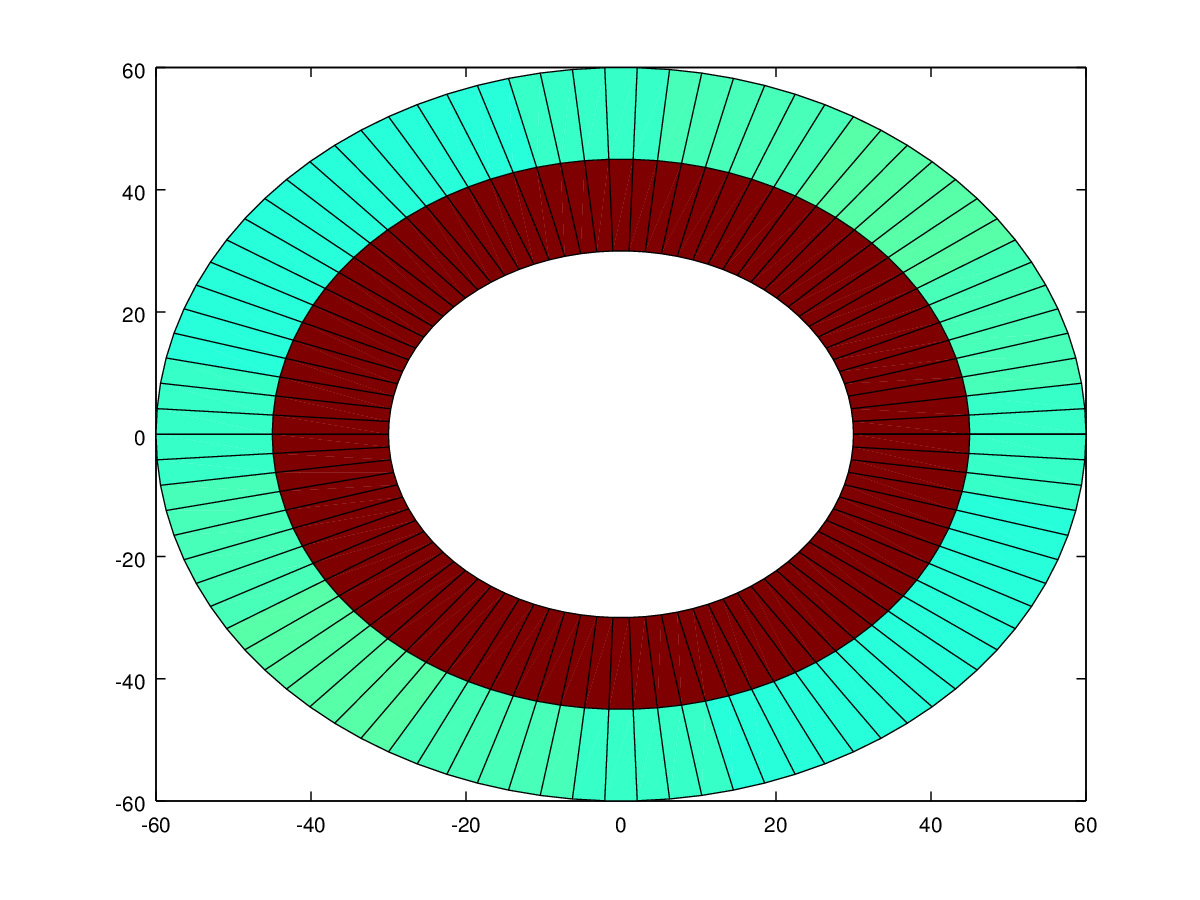
\includegraphics[width=4.5cm]{graficos/exp4/seno/exp4-seno-rad-3.png} &
              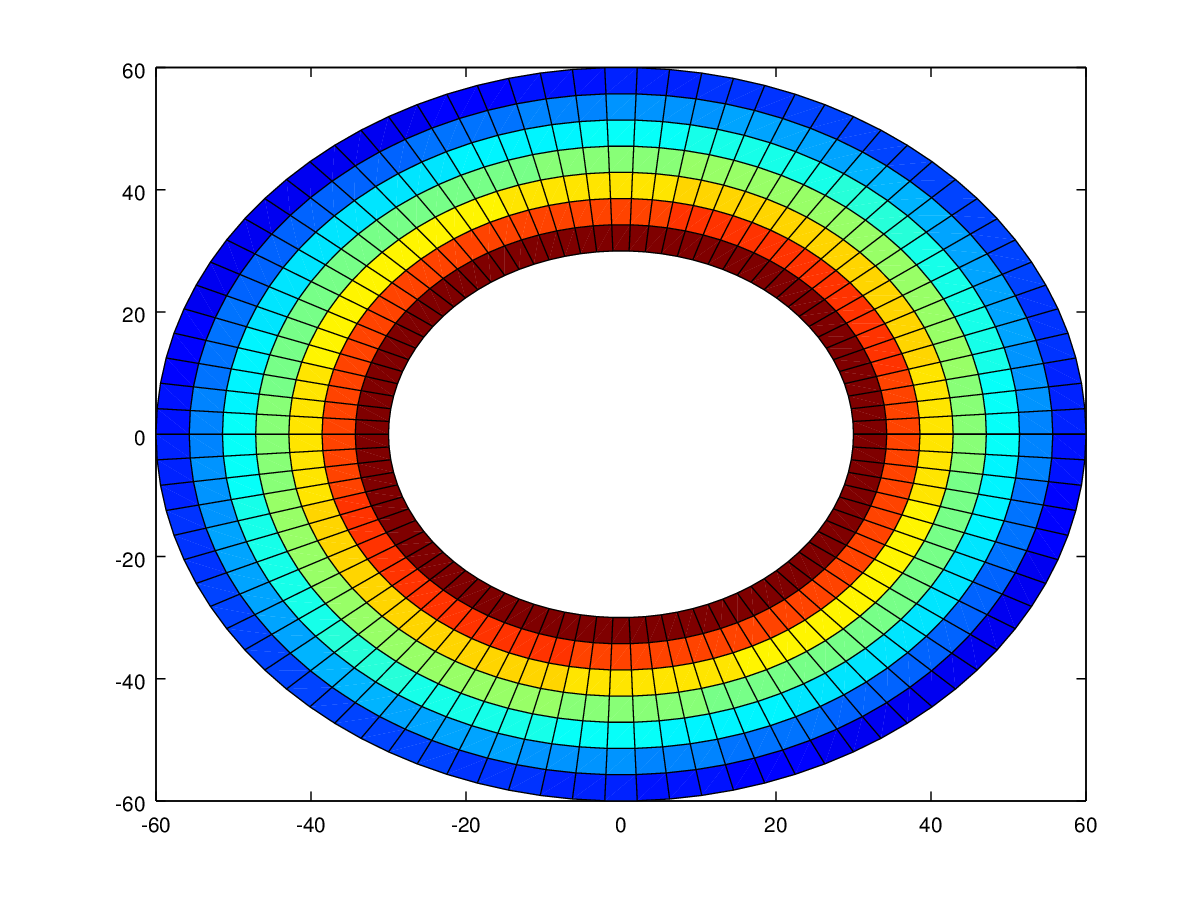
\includegraphics[width=4.5cm]{graficos/exp4/seno/exp4-seno-rad-8.png} &
              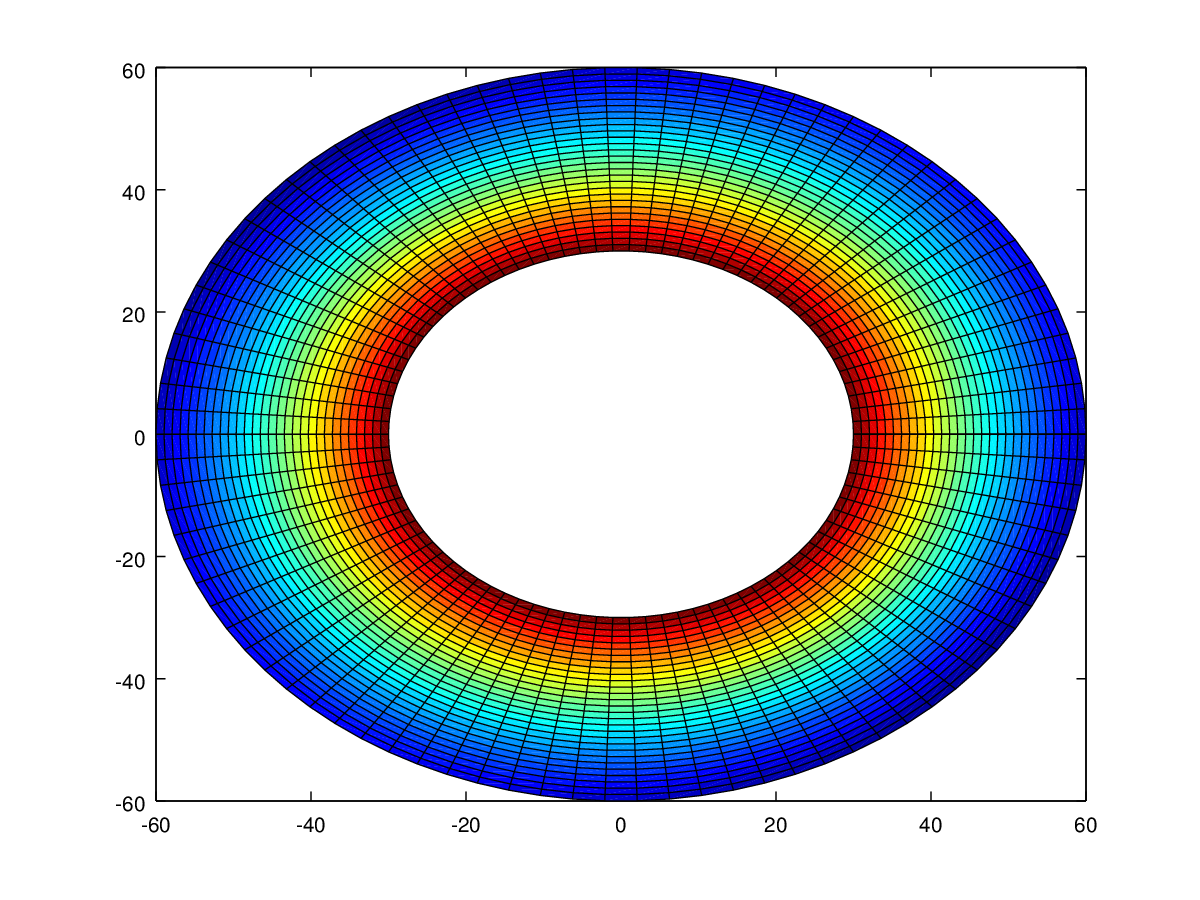
\includegraphics[width=4.5cm]{graficos/exp4/seno/exp4-seno-rad-30.png} \\
              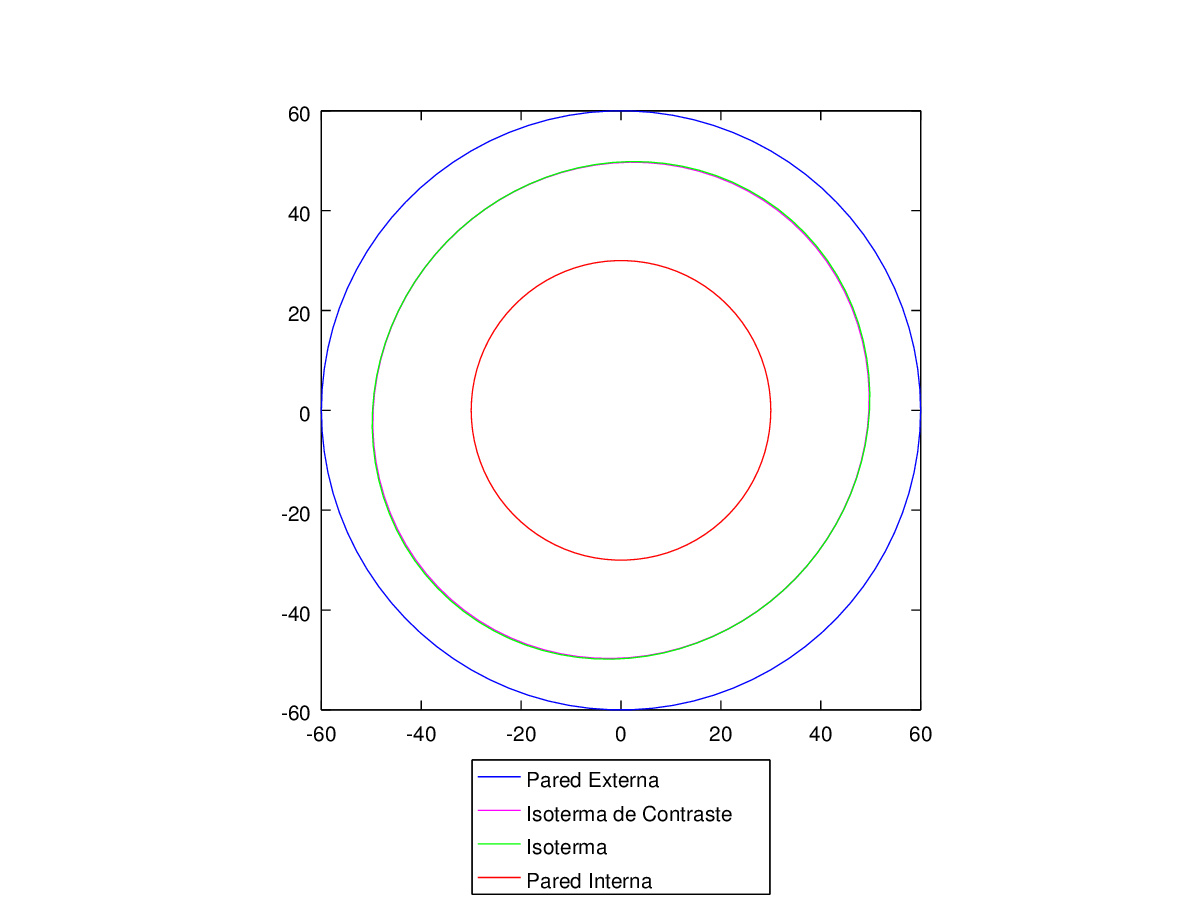
\includegraphics[width=5cm]{graficos/exp4/seno/exp4-seno-rad-3-iso.png} &
              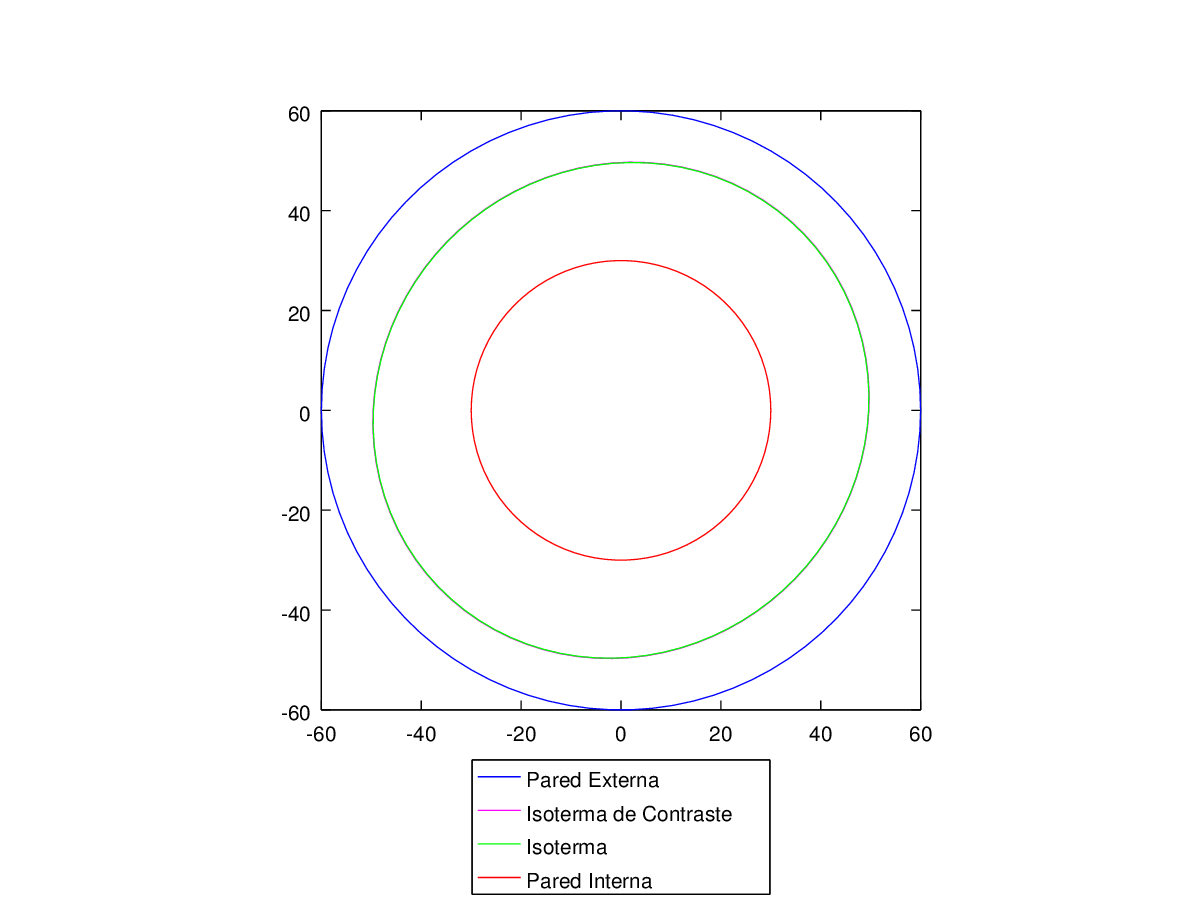
\includegraphics[width=5cm]{graficos/exp4/seno/exp4-seno-rad-8-iso.png} &
              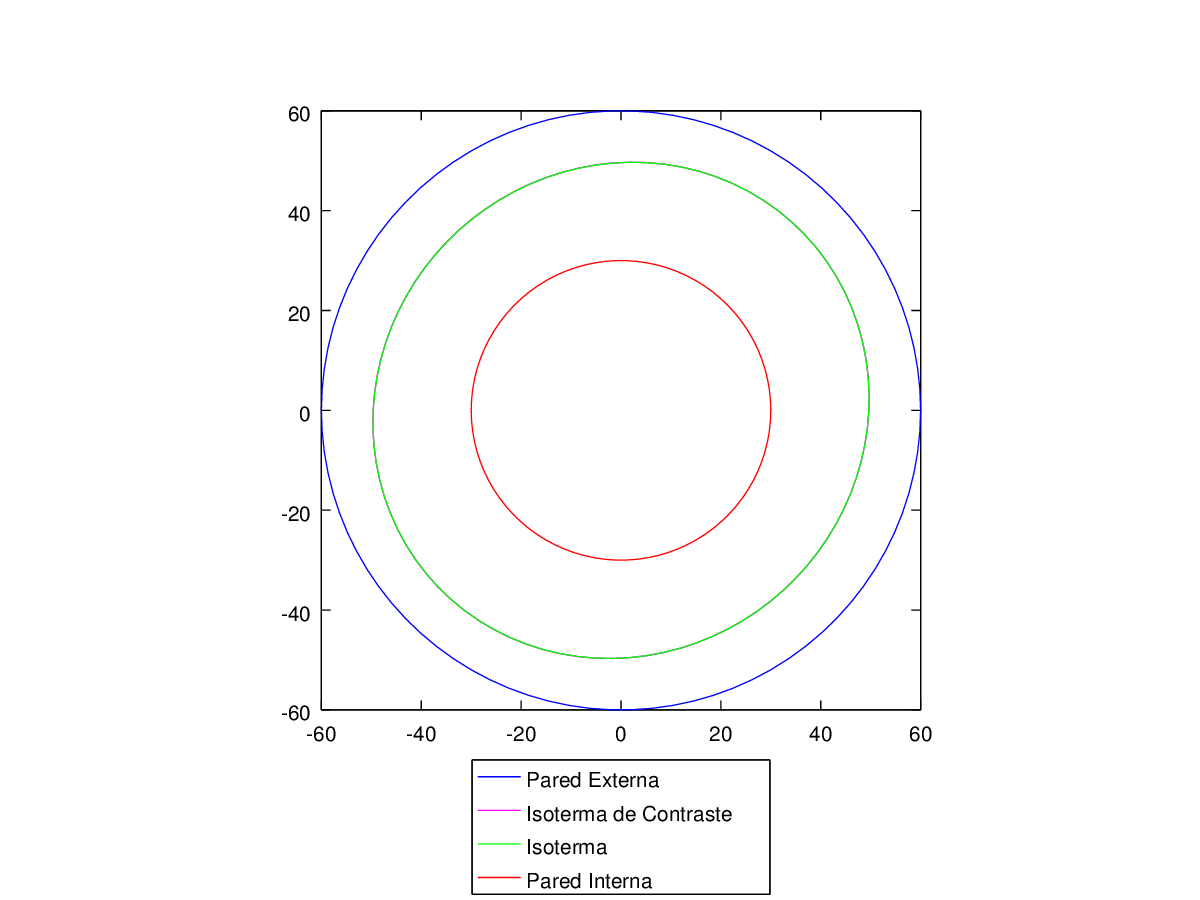
\includegraphics[width=5cm]{graficos/exp4/seno/exp4-seno-rad-30-iso.png} \\
              {\small $m+1 = 3$} &
              {\small $m+1 = 8$} &
              {\small $m+1 = 30$} \\
            \end{tabular}}

      \subsubsection*{Discusión}
        Como se puede observar en los resultados, variar la granularidad con respecto a los ángulos no afecta al resultado de la posición de la isoterma. Ésta sigue siendo igual que la de contraste. Cuanto mayor cantidad de ángulos se tengan, más información podrá verse pero sin afectar el resultado total. En cambio, cuando modificamos la granularidad con respecto a los radios la isoterma calculada se aleja de la de contraste. Dejamos a experimento futuro observar que tanto se modifica dependiendo de las temperaturas de la pared externa del horno. Para ello podíamos tomar valores de temperaturas externas mayores que 200 grados y menores que 50 grados a modo de análisis.


    \subsubsection*{Experimento 5: Índice de peligrosidad según ancho de la pared}

      \subsubsection*{Presentación}
        Se busca estudiar la variación de la medida de peligrosidad con respecto al grosor de la pared del alto horno, sin modificar las temperaturas de la pared externa. Para ello modificaremos el radio interno dejando constante el externo. Se realizará de esta manera ya que para lo que se quiere observar es indistinto cual de los dos variar. 

      \subsubsection*{Datos}
        Para este experimento se mantuvieron constantes los parámetros, $r_e = 90$, $m+1 = 30$, $n = 80$, $T_i = 1500$, $iso = 500$, como así también la temperatura externa $T_e(\theta)$, para la cual se tomaron valores arbitrarios entre 50 y 200{\degree}C. Se generaron instancias con los siguientes valores de $r_i$: $5, 10, 20, 40, 60, 80, 90$.  Se puede encontrar en los archivos adjuntos llamados exp5-$r_i$.in la instancia pasada por parámetro.
     
      \subsubsection*{Hipótesis}
        La hipótesis de este experimento es que a medida que el grosor de la pared disminuye, el índice de peligrosidad aumenta. Suponemos que esto se debe a que al dejar las temperaturas constantes, la isoterma se encuentra cada vez más cerca de la pared externa.
        
      \subsubsection*{Resultados}

        En el gráfico pueden observarse los valores obtenidos para el índice de peligrosidad en función de los diferentes valores de $r_i$.

          \begin{center}
            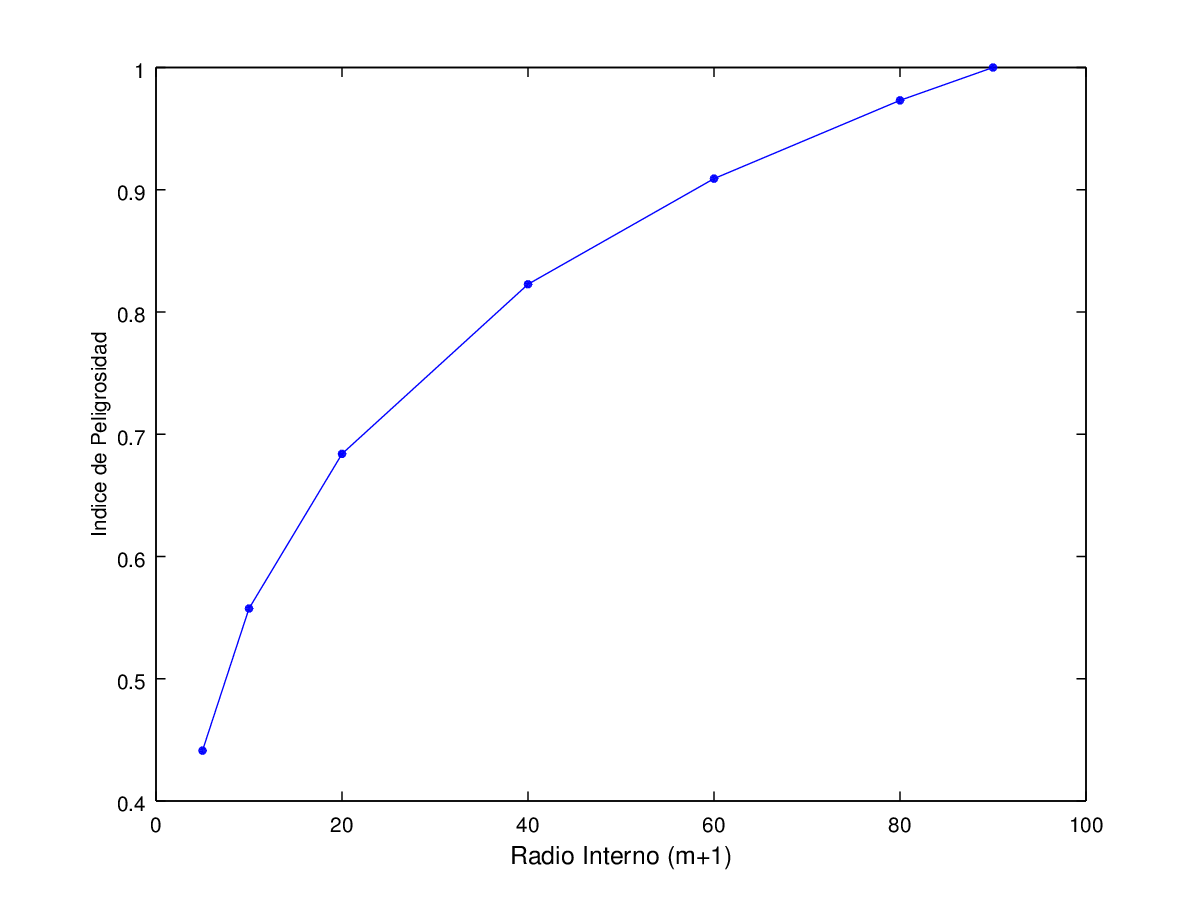
\includegraphics[width=9cm]{graficos/exp5/exp5.png} \\
            {\small Índice de peligrosidad en función del valor de $r_i$}
          \end{center}

      \subsubsection*{Discusión}
        En este experimento se puede ver que a medida que disminuimos el grosor de la pared del alto horno la isoterma se encuentra cada vez mas cerca de la pared externa. El índice de peligrosidad mide la relación entre la temperatura más alta y la proximidad de la misma a la pared externa. 
        Cuando disminuimos el grosor de la pared, lo que hacemos es acercar la pared interna (donde se encuentra la temperatura más alta del sistema) a la pared externa. De esta forma la isoterma va a estar mas próxima a la pared externa que cuando el grosor es mayor. Entonces el índice de peligrosidad aumentará, demostrando así lo que se planteó en la hipótesis.

\clearpage
\section{Conclusiones}

  Además de exponer otra de las tantas posibilidades de aplicación a problemas físicos de la resolución de sistemas de ecuaciones lineales, la realización de este trabajo permitió, a partir de las pruebas experimentales llevadas a cabo, extraer las siguientes conclusiones con respecto a los dos aspectos del problema cubiertos por estas pruebas: el rendimiento de los métodos y el comportamiento del sistema.

  Las comparaciones realizadas entre los métodos estudiados con respecto a su rendimiento temporal muestran que este fue muy similar entre ambos cuando solo se realizó el cálculo para una única instancia. Sin embargo, al realizar el cálculo repetidamente para varias instancias, manteniendo constantes los parámetros del problema pero variando los datos de entrada, el método de Factorización LU se mostró claramente superior al de Eliminación Gaussiana. Dado que este escenario podría presentarse en el caso de aplicación estudiado, por ejemplo, al analizar la evolución temporal del sistema, la utilización del método de Factorización LU podría ser convieniente.

  Cabe destacar también que el aumento de la granularidad de la discretización repercute negativamente en el rendimiento de ambos métodos por igual. Esto indica que debe estudiarse con cuidado la granularidad necesaria, considerando las limitaciones particulares del contexto a la hora de realizar los cálculos.

  En cuanto al comportamiento del sistema, se pudieron verificar las hipótesis de que la cercanía de la isoterma en el interior de la pared del horno es directamente proporcional a la temperatura externa e inversamente proporcional al grosor de la pared del horno. Esto arroja información que puede ser útil a la hora de prevenir situaciones de riesgo en el contexto de aplicación real. Por otra parte, se comprobó que la precisión de la estimación de la posición de la isoterma es más sensible a cambios en la granularidad de radios que de ángulos; no obstante, sería útil continuar experimentando para verificar el efecto que una menor granularidad de ángulos puede tener en el índice de peligrosidad y en la detección de situaciones de riesgo.

\clearpage

% Apéndices
\begin{appendices}
  \section{Enunciado del trabajo práctico}

  \subsection{Introducción}

    Consideremos la sección horizontal de un horno de acero cilíndrico, como en la Figura \ref{fig:seccionHorno}. El sector A es la pared del horno, y el sector B es el horno propiamente dicho, en el cual se funde el acero a temperaturas elevadas. Tanto el borde externo como el borde interno de la pared forman círculos. Suponemos que la temperatura del acero dentro del horno (o sea, dentro de B) es constante e igual a 1500{\degree}C.
    Tenemos sensores ubicados en la parte externa del horno para medir la temperatura de la pared externa del mismo, que habitualmente se encuentra entre 50{\degree}C y 200{\degree}C. El problema que debemos resolver consiste en estimar la isoterma de 500{\degree}C dentro de la pared del horno, para estimar la resistencia de la misma. Si esta isoterma está demasiado cerca de la pared externa del horno, existe peligro de que la estructura externa de la pared colapse.

    \begin{figure}[h]
      \centering
      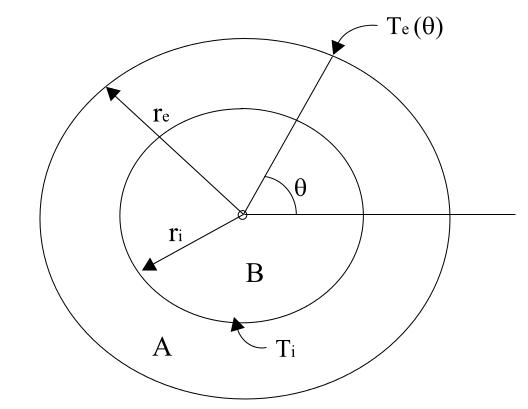
\includegraphics[width=10cm]{seccionHorno.jpg}
      \caption{Sección circular del horno.}
      \label{fig:seccionHorno}
    \end{figure}

    El objetivo del trabajo práctico es implementar un programa que calcule la isoterma solicitada, conociendo las dimensiones del horno y las mediciones de temperatura en la pared exterior.

  \subsection{El Modelo}

    Sea $r_e \in \mathbb{R}$ el radio exterior de la pared y sea $r_i \in \mathbb{R}$ el radio interior de la pared. Llamemos $T(r, \theta)$ a la temperatura en el punto dado por las coordenadas polares $(r, \theta)$, siendo $r$ el radio y $\theta$ el ángulo polar de dicho punto. En el estado estacionario, esta temperatura satisface la ecuación del calor:

    \begin{equation} \label{eq:en1}
      \frac{\partial^2 T(r, \theta)}{\partial r^2} + \frac{1}{r} \frac{\partial T(r, \theta)}{\partial r} + \frac{1}{r^2} \frac{\partial^2 T(r, \theta)}{\partial \theta^2} = 0
    \end{equation}

    Si llamamos $T_i \in \mathbb{R}$ a la temperatura en el interior del horno (sector B) y $T_e : [0, 2\pi] \to \mathbb{R}$ a la función de temperatura en el borde exterior del horno (de modo tal que el punto $(r_e, \theta)$ tiene temperatura $T_e(\theta)$), entonces tenemos que

    \begin{equation} \label{eq:en2}
      T(r, \theta) = T_i \text{ para todo punto } (r, \theta) \text{ con } r \leq r_i
    \end{equation}

    \begin{equation} \label{eq:en3}
      T(r_e, \theta) = T_e(\theta) \text{ para todo punto } (r_e, \theta)
    \end{equation}

    El problema en derivadas parciales dado por la primera ecuación con las condiciones de contorno presentadas recientemente, permite encontrar la función $T$ de temperatura en el interior del horno (sector A), en función de los datos mencionados en esta sección.

    Para resolver este problema computacionalmente, discretizamos el dominio del problema (el sector A) en coordenadas polares. Consideramos una partición $0 = \theta_0 < \theta_1 < ... < \theta_n = 2\pi$ en $n$ ángulos discretos con $\theta_k - \theta_{k-1} = \Delta \theta$ para $k = 1, \dots n$, y una partición $r_i = r_0 < r_1 < ... < r_m = r_e$ en $m + 1$ radios discretos con $r_j - r_{j-1} = \Delta r$ para $j = 1, \dots m$.

    El problema ahora consiste en determinar el valor de la función $T$ en los puntos de la discretización $(r_j, \theta_k)$ que se encuentren dentro del sector A. Llamemos $t_{jk} = T(r_j , \theta_k)$ al valor (desconocido) de la función $T$ en el punto $(r_j, \theta_k)$.

    Para encontrar estos valores, transformamos la ecuación (\ref{eq:en1}) en un conjunto de ecuaciones lineales sobre las incógnitas $t_{jk}$, evaluando (\ref{eq:en1}) en todos los puntos de la discretización que se encuentren dentro del sector A. Al hacer esta evaluación, aproximamos las derivadas parciales de $T$ en (\ref{eq:en1}) por medio de las siguientes fórmulas de diferencias finitas:

    \begin{equation} \label{eq:en4}
      \frac{\partial^2 T(r, \theta)}{\partial r^2}(r_j, \theta_k) \cong \frac{t_{j-1,k} - 2 t_{jk} + t_{j+1,k}}{(\Delta r)^2}
    \end{equation}

    \begin{equation} \label{eq:en5}
      \frac{\partial T(r, \theta)}{\partial r}(r_j, \theta_k) \cong \frac{t_{j,k} - t_{j-1,k}}{\Delta r}
    \end{equation}

    \begin{equation} \label{eq:en6}
      \frac{\partial^2 T(r, \theta)}{\partial \theta^2}(r_j, \theta_k) \cong \frac{t_{j,k-1} - 2 t_{jk} + t_{j,k+1}}{(\Delta \theta)^2}
    \end{equation}

    Es importante notar que los valores de las incógnitas son conocidos para los puntos que se encuentran sobre el borde exterior de la pared, y para los puntos que se encuentren dentro del sector B. Al realizar este procedimiento, obtenemos un sistema de ecuaciones lineales que modela el problema discretizado. La resolución de este sistema permite obtener una aproximación de los valores de la función $T$ en los puntos de la discretización.

  \subsection{Enunciado}
    Se debe implementar un programa en \texttt{C} o \texttt{C++} que tome como entrada los parámetros del problema ($r_i$, $r_e$, $m + 1$, $n$, valor de la isoterma buscada, $T_i$, $T_e(\theta)$) que calcule la temperatura dentro de la pared del horno utilizando el modelo propuesto en la sección anterior y que encuentre la isoterma buscada en función del resultado obtenido del sistema de ecuaciones. El método para determinar la posición de la isoterma queda a libre elección de cada grupo y debe ser explicado en detalle en el informe.

    El programa debe formular el sistema obtenido a partir de las ecuaciones (\ref{eq:en1})-(\ref{eq:en6}) y considerar dos métodos posibles para su resolución: mediante el algoritmo clásico de Eliminación Gaussiana y la Factorización LU. Finalmente, el programa escribirá en un archivo la solución obtenida con el formato especificado en la siguiente sección.

    Como ya se ha visto en la materia, no es posible aplicar los métodos propuestos para la resolución a cualquier sistema de ecuaciones. Sin embargo, la matriz del sistema considerado en el presente trabajo cumple con ser diagonal dominante (no estricto) y que, ordenando las variables y ecuaciones convenientemente, es posible armar un sistema de ecuaciones cuya matriz posee la propiedad de ser \emph{banda}. Luego, se pide demostrar (o al menos dar un esquema de la demostración) el siguiente resultado e incluirlo en el informe:

    \begin{prop}
      Sea $A \in \mathbb{R}^{n \times n}$ la matriz obtenida para el sistema definido por (\ref{eq:en1})-(\ref{eq:en6}). Demostrar que es posible aplicar Eliminación Gaussiana sin pivoteo.\footnote{Sugerencia: Notar que la matriz es diagonal dominante (no estrictamente) y analizar qué sucede al aplicar un paso de Eliminación Gaussiana con los elementos de una fila.}
    \end{prop}

    La solución del sistema de ecuaciones permitirá saber la temperatura en los puntos de la discretización. Sin embargo, nuestro interés es calcular la isoterma 500, para poder determinar si la estructura se encuentra en peligro. Luego, se pide lo siguiente:

    \begin{itemize}
      \item Dada la solución del sistema de ecuaciones, proponer una forma de estimar en cada ángulo de la discretización la posición de la isoterma 500.
      \item En función de la aproximación de la isoterma, proponer una forma (o medida) a utilizar para evaluar la peligrosidad de la estructura en función de la distancia a la pared externa del horno.
    \end{itemize}

    En función de la experimentación, se busca realizar dos estudios complementarios: por un lado, analizar cómo se comporta el sistema y, por otro, cuáles son los requerimientos computacionales de los métodos. Se pide como mínimo realizar los siguientes experimentos:

    \begin{enumerate}
      \item Comportamiento del sistema.
        \begin{itemize}
          \item Considerar al menos dos instancias de prueba, generando distintas discretizaciones para cada una de ellas y comparando la ubicación de la isoterma buscada respecto de la pared externa del horno. Se sugiere presentar gráficos de temperatura o curvas de nivel para los mismos, ya sea utilizando las herramientas provistas por la cátedra o implementando sus propias herramientas de graficación.
          \item Estudiar la proximidad de la isoterma buscada respecto de la pared exterior del horno en función de distintas granularidades de discretización y las condiciones de borde.
        \end{itemize}

      \item Evaluación de los métodos.
        \begin{itemize}
          \item Analizar el tiempo de cómputo requerido para obtener la solución del sistema en función de la granularidad de la discretización. Se sugiere presentar los resultados mediante gráficos de tiempo de cómputo en función de alguna de las variables del problema.
          \item Considerar un escenario similar al propuesto en el experimento 1. pero donde las condiciones de borde (i.e., $T_i$ y $T_e(\theta)$) cambian en distintos instantes de tiempo. En este caso, buscamos obtener la secuencia de estados de la temperatura en la pared del horno, y la respectiva ubicación de la isoterma especificada. Para ello, se considera una secuencia de $ninst$ vectores con las condiciones de borde, y las temperaturas en cada estado es la solución del correspondiente sistema de ecuaciones. Se pide formular al menos un experimento de este tipo, aplicar los métodos de resolución propuestos de forma conveniente y compararlos en términos de tiempo total de cómputo requerido para distintos valores de $ninst$.
        \end{itemize}
    \end{enumerate}

    De manera opcional, aquellos grupos que quieran ir un poco más allá pueden considerar trabajar y desarrollar alguno(s) de los siguientes puntos extra:
    \begin{enumerate}
      \item Notar que el sistema resultante tiene estructura \emph{banda}. Proponer una estructura para aprovechar este hecho en términos de la \emph{complejidad espacial} y como se adaptarían los algoritmos de Eliminación Gaussiana y Factorización LU para reducir la cantidad de operaciones a realizar.
      \item Implementar dicha estructura y las adaptaciones necesarias para el algoritmo de Eliminación Gaussiana.
      \item Implementar dicha estructura y las adaptaciones necesarias para el algoritmo de Factorización LU.
    \end{enumerate}

    Finalmente, se deberá presentar un informe que incluya una descripción detallada de los métodos implementados y las decisiones tomadas, el método propuesto para el cálculo de la isoterma buscada y los experimentos realizados, junto con el correspondiente análisis y siguiendo las pautas definidas en el archivo \texttt{pautas.pdf}.

  \subsection{Programa y formato de archivos}
    Se deberán entregar los archivos fuentes que contengan la resolución del trabajo práctico. El ejecutable tomará tres parámetros por línea de comando, que serán el archivo de entrada, el archivo de salida, y el método a ejectutar (0 Eliminación Gaussiana, 1 LU).

    El archivo de entrada tendrá la siguiente estructura:
    \begin{itemize}
      \item La primera línea contendrá los valores $r_i$, $r_e$, $m + 1$, n, iso, $ninst$, donde $iso$ representa el valor de la isoterma buscada y $ninst$ es la cantidad de instancias del problema a resolver para los parámetros dados.
      \item A continuación, el archivo contendrá $ninst$ líneas, cada una de ellas con $2 n$ valores, los primeros $n$ indicando los valores de la temperatura en la pared interna, i.e., $T_i(\theta_0), T_i(\theta_1), \dots, T_i(\theta_n-1)$, seguidos de $n$ valores de la temperatura en la pared externa, i.e., $T_e(\theta_0), T_e(\theta_1), \dots, T_e(\theta_n-1)$.
    \end{itemize}

    El archivo de salida obligatorio tendrá el vector solución del sistema reportando una componente del mismo por línea. En caso de $ninst > 1$, los vectores serán reportados uno debajo del otro.

    Junto con el presente enunciado, se adjunta una serie de scripts hechos en \texttt{python} y un conjunto instancias de test que deberán ser utilizados para la compilación y un testeo básico de la implementación. Se recomienda leer el archivo \texttt{README.txt} con el detalle sobre su utilización.

  \subsection{Fechas de entrega}
    \begin{itemize}
      \item \emph{Formato Electrónico}: Jueves 3 de Septiembre de 2015, hasta las 23:59 hs, enviando el trabajo (informe + código) a la dirección \texttt{metnum.lab@gmail.com}. El subject del email debe comenzar con el texto \texttt{[TP1]} seguido de la lista de apellidos de los integrantes del grupo.
      \item \emph{Formato físico}: Viernes 4 de Septiembre de 2015, de 17:30 a 18:00 hs.
    \end{itemize}

    \strong{Importante}: El horario es estricto. Los correos recibidos después de la hora indicada serán considerados re-entrega. Los grupos deben ser de 3 o 4 personas, sin excepción. Es indispensable que los trabajos pasen satisfactoriamente los casos de test provistos por la cátedra.

  \clearpage
\end{appendices}

% Referencias
\printbibliography[heading=bibintoc]

\end{document}
